\section{Part 1A: Vowel Formant Analysis}

\subsection{Overview}

In this part, you will analyze recordings of speakers of American English uttering the following words:

\begin{enumerate}
\item heed -- [h i\textlengthmark{} d]
\item hid -- [h \textsci{} d]
\item head -- [h \textepsilon{} d] 
\item had -- [h \ae{} d]
\item hod -- [h \textscripta\textlengthmark{} d]
\item hawed -- [h \textopeno\textlengthmark{} d]
\item hood -- [h \textupsilon{} d]
\item who'd -- [h u\textlengthmark{} d]
\end{enumerate}

Your task will be to measure the values of the first two formants (i.e., resonant frequencies of the human voice), F1 and F2, for the sounds produced by one speaker, and create a scatter plot of their F1 and F2 values, with F2 in the x--axis and F1 in the y--axis.

In addition, you will replot the same data in the context of an older database of F1 and F2 values collected by \citeA{peterson1952} to compare the values observed in a single individual with those of a larger group of people.

\subsection{What you will need}

In order to complete this part of the lab, you will need:

\begin{enumerate}
\item the sound files
\item the software \Praat{}, for the formant analysis and data plotting
\item a spreadsheet program --- \Gsheet{}, \MSExcel{}, or \OpOff{} are fine options --- to store the values you measure.
\end{enumerate}

\subsubsection{The sound files}

The sound files are available in the compressed folder for this lab, and come from a large study of American English vowels by \citeA{hillenbrand1995}. The folders \emph{men} and \emph{women} contain the recordings done by \citeA{hillenbrand1995} for 50 men and 50 women. Each uttered one of the 12 American English vowels in a h\_V\_d context. In this lab, we will only analyze the eight vowels enumerated in the previous section.

Each sound file is coded in the following manner:

\begin{itemize}
\item the first letter indicates whether the speaker is male (\emph{m}) of female (\emph{w})
\item the numbers after the first letter indicate the participant's code (1--50)
\item the next two letters indicate the vowel that is pronounced in the sound file, which are:
    \begin{itemize}
    \item ae=``had'';[\ae{}]
    \item ah=``hod''; [\textscripta{}]
    \item aw=``hawed''; [\textopeno{}]
    \item eh=``head''; [\textepsilon{}]
    \item er=``heard''; [\textrhookschwa{}]
    \item ei=``haid''; [e]
    \item ih=``hid''; [\textsci{}]
    \item iy=``heed''; [i]
    \item oa=/o/ as in ``boat''; [o]
    \item oo=``hood''; [\textupsilon{}]
    \item uh=``hud''; [\textturnv]
    \item uw=``who'd''; [u]
    \end{itemize}
\end{itemize}

Your goal will be to select one participant at random and measure the formants F1 and F2 values for a subset of the vowels above, repeated below with the coding used in the file names:

\begin{enumerate}
\item heed -- [h i\textlengthmark{} d] -- iy
\item hid -- [h \textsci{} d] -- ih
\item head -- [h \textepsilon{} d] -- eh
\item had -- [h \ae{} d] -- ae
\item hod -- [h \textscripta\textlengthmark{} d] -- ah
\item hawed -- [h \textopeno\textlengthmark{} d] -- aw
\item hood -- [h \textupsilon{} d] -- uh
\item who'd -- [h u\textlengthmark{} d] -- uw
\end{enumerate}

\paragraph{How to select the sound files to analyze?} First, you will need to pick a random number between 1--50. You will also pick a male speaker if you are male and a female speaker if you are female. For instance, if you are female, and you picked the number 33, you would analyze the following files in the \emph{women} folder:

\begin{enumerate}
\item \filefmat{w33iy.wav}
\item \filefmat{w33ih.wav}
\item \filefmat{w33eh.wav}
\item \filefmat{w33ae.wav}
\item \filefmat{w33ah.wav}
\item \filefmat{w33aw.wav}
\item \filefmat{w33uh.wav}
\item \filefmat{w33uw.wav}
\end{enumerate}

\subsubsection{Using \Praat{} to measure the formant values}

\paragraph{Opening \Praat{}.} The first thing you need to do is open \Praat{}. You should see two separate windows, called \filefmat{Praat Objects} and \filefmat{Praat Picture}, as shown in figure~\ref{praat-main-windows}:

\begin{figure}[!tbp]
\caption{\Praat{} -- Main Windows}
\label{praat-main-windows}
	\begin{center}
		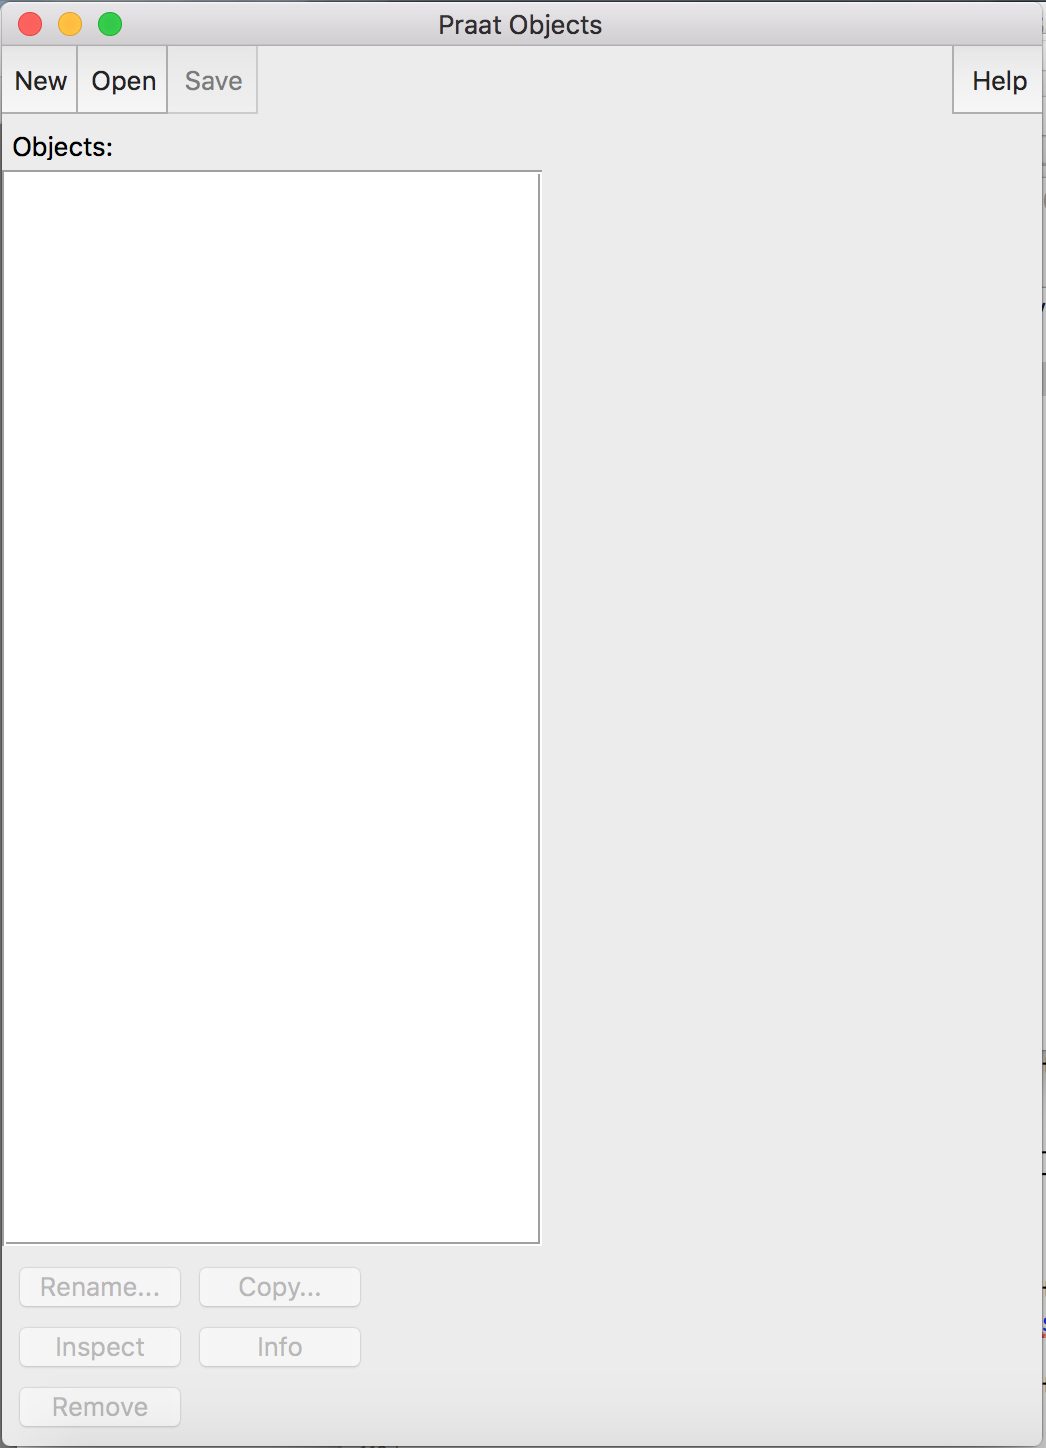
\includegraphics[width=0.45\textwidth]{./figures/Praat-01-Objects-Window}
		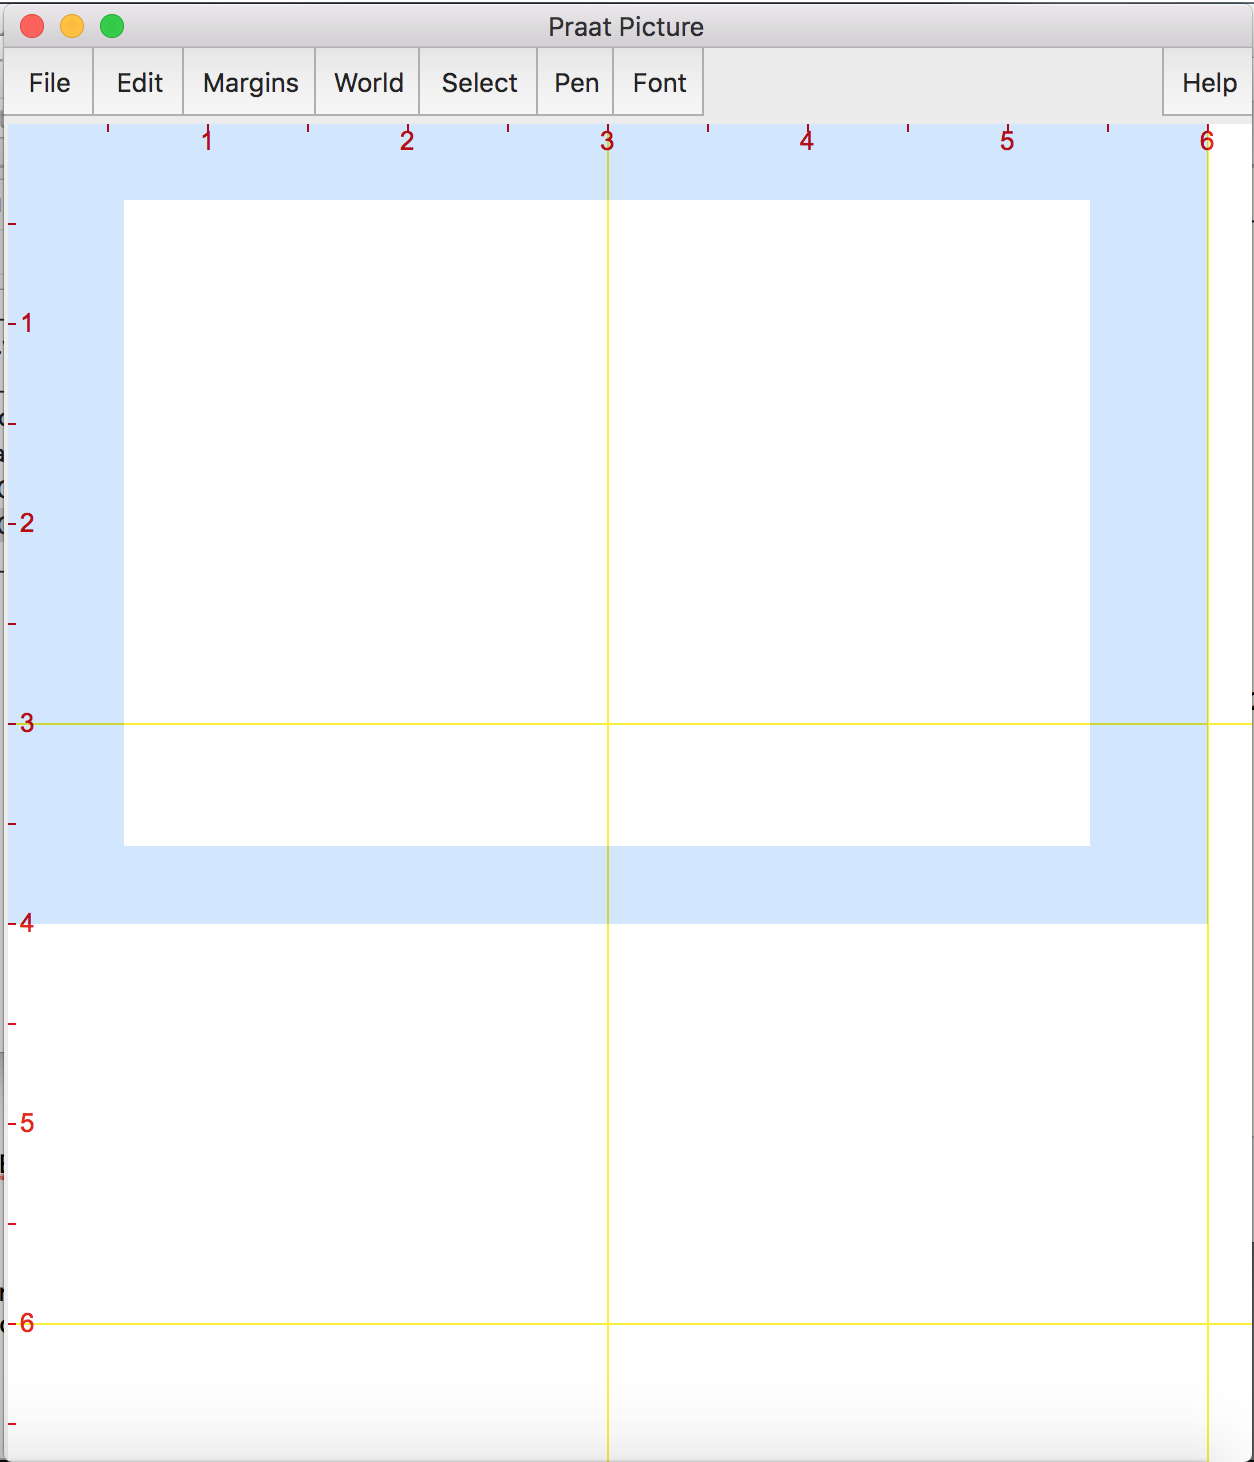
\includegraphics[width=0.45\textwidth]{./figures/Praat-02-Picture-Window}
	\end{center}
\end{figure}

\paragraph{Loading a file.} In the \filefmat{Objects} window, click on \softmenu{Open} $>$ \softmenu{Read from file}, as shown in figure~\ref{praat-read-from-file}:

\begin{figure}[!tbp]
\caption{\Praat{} -- Reading from a file}
\label{praat-read-from-file}
	\begin{center}
		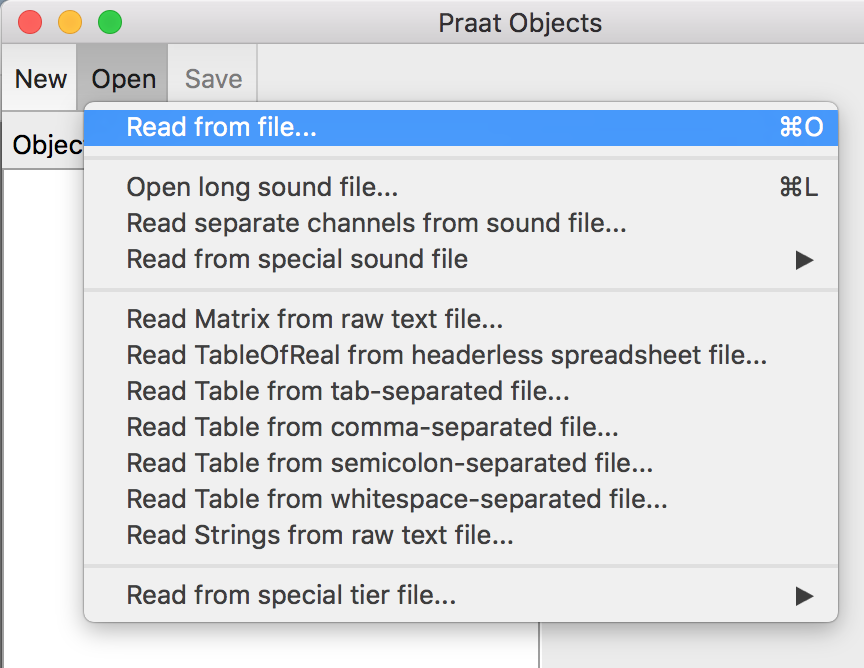
\includegraphics[width=0.8\textwidth]{./figures/Praat-03-Read-from-file}
	\end{center}
\end{figure}

Once you select the file you want to open and click on it, its name should appear in the \filefmat{Objects} window, as shown in figure~\ref{praat-object-in-list}.

\begin{figure}[!tbp]
\caption{\Praat{} -- Object in List}
\label{praat-object-in-list}
	\begin{center}
		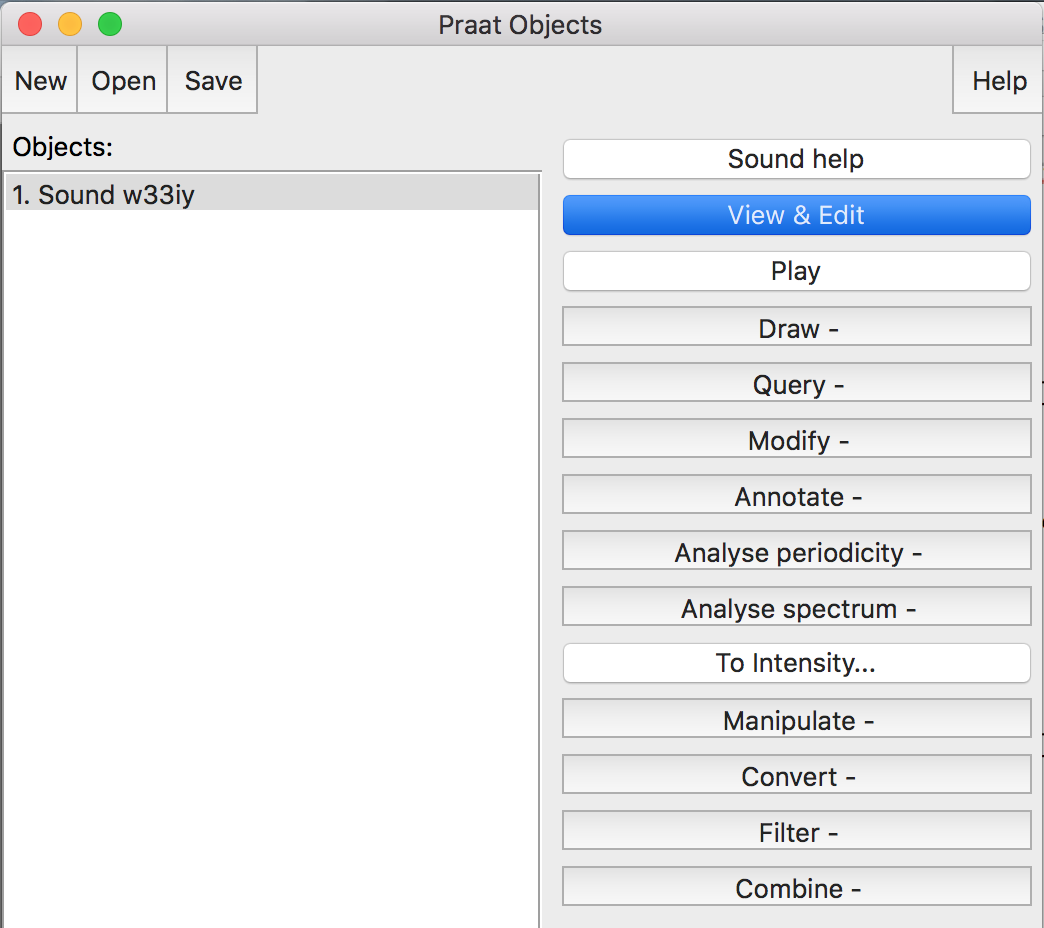
\includegraphics[width=0.8\textwidth]{./figures/Praat-04-Object-in-list}
	\end{center}
\end{figure}

Notice how the button \softmenu{View \& Edit} has automatically highlighted for you.


\paragraph{Looking at the spectrogram.} Once you have read the appropriate file into \Praat{}, you should be able to see it on your object list (figure~\ref{praat-object-in-list}), and the button \softmenu{View \& Edit} has automatically been highlighted for you. If you click on it, it should open the sound editor window, as shown in figure~\ref{praat-view-and-edit}.

\begin{figure}[!tbp]
\caption{\Praat{} -- View and Edit Window}
\label{praat-view-and-edit}
	\begin{center}
		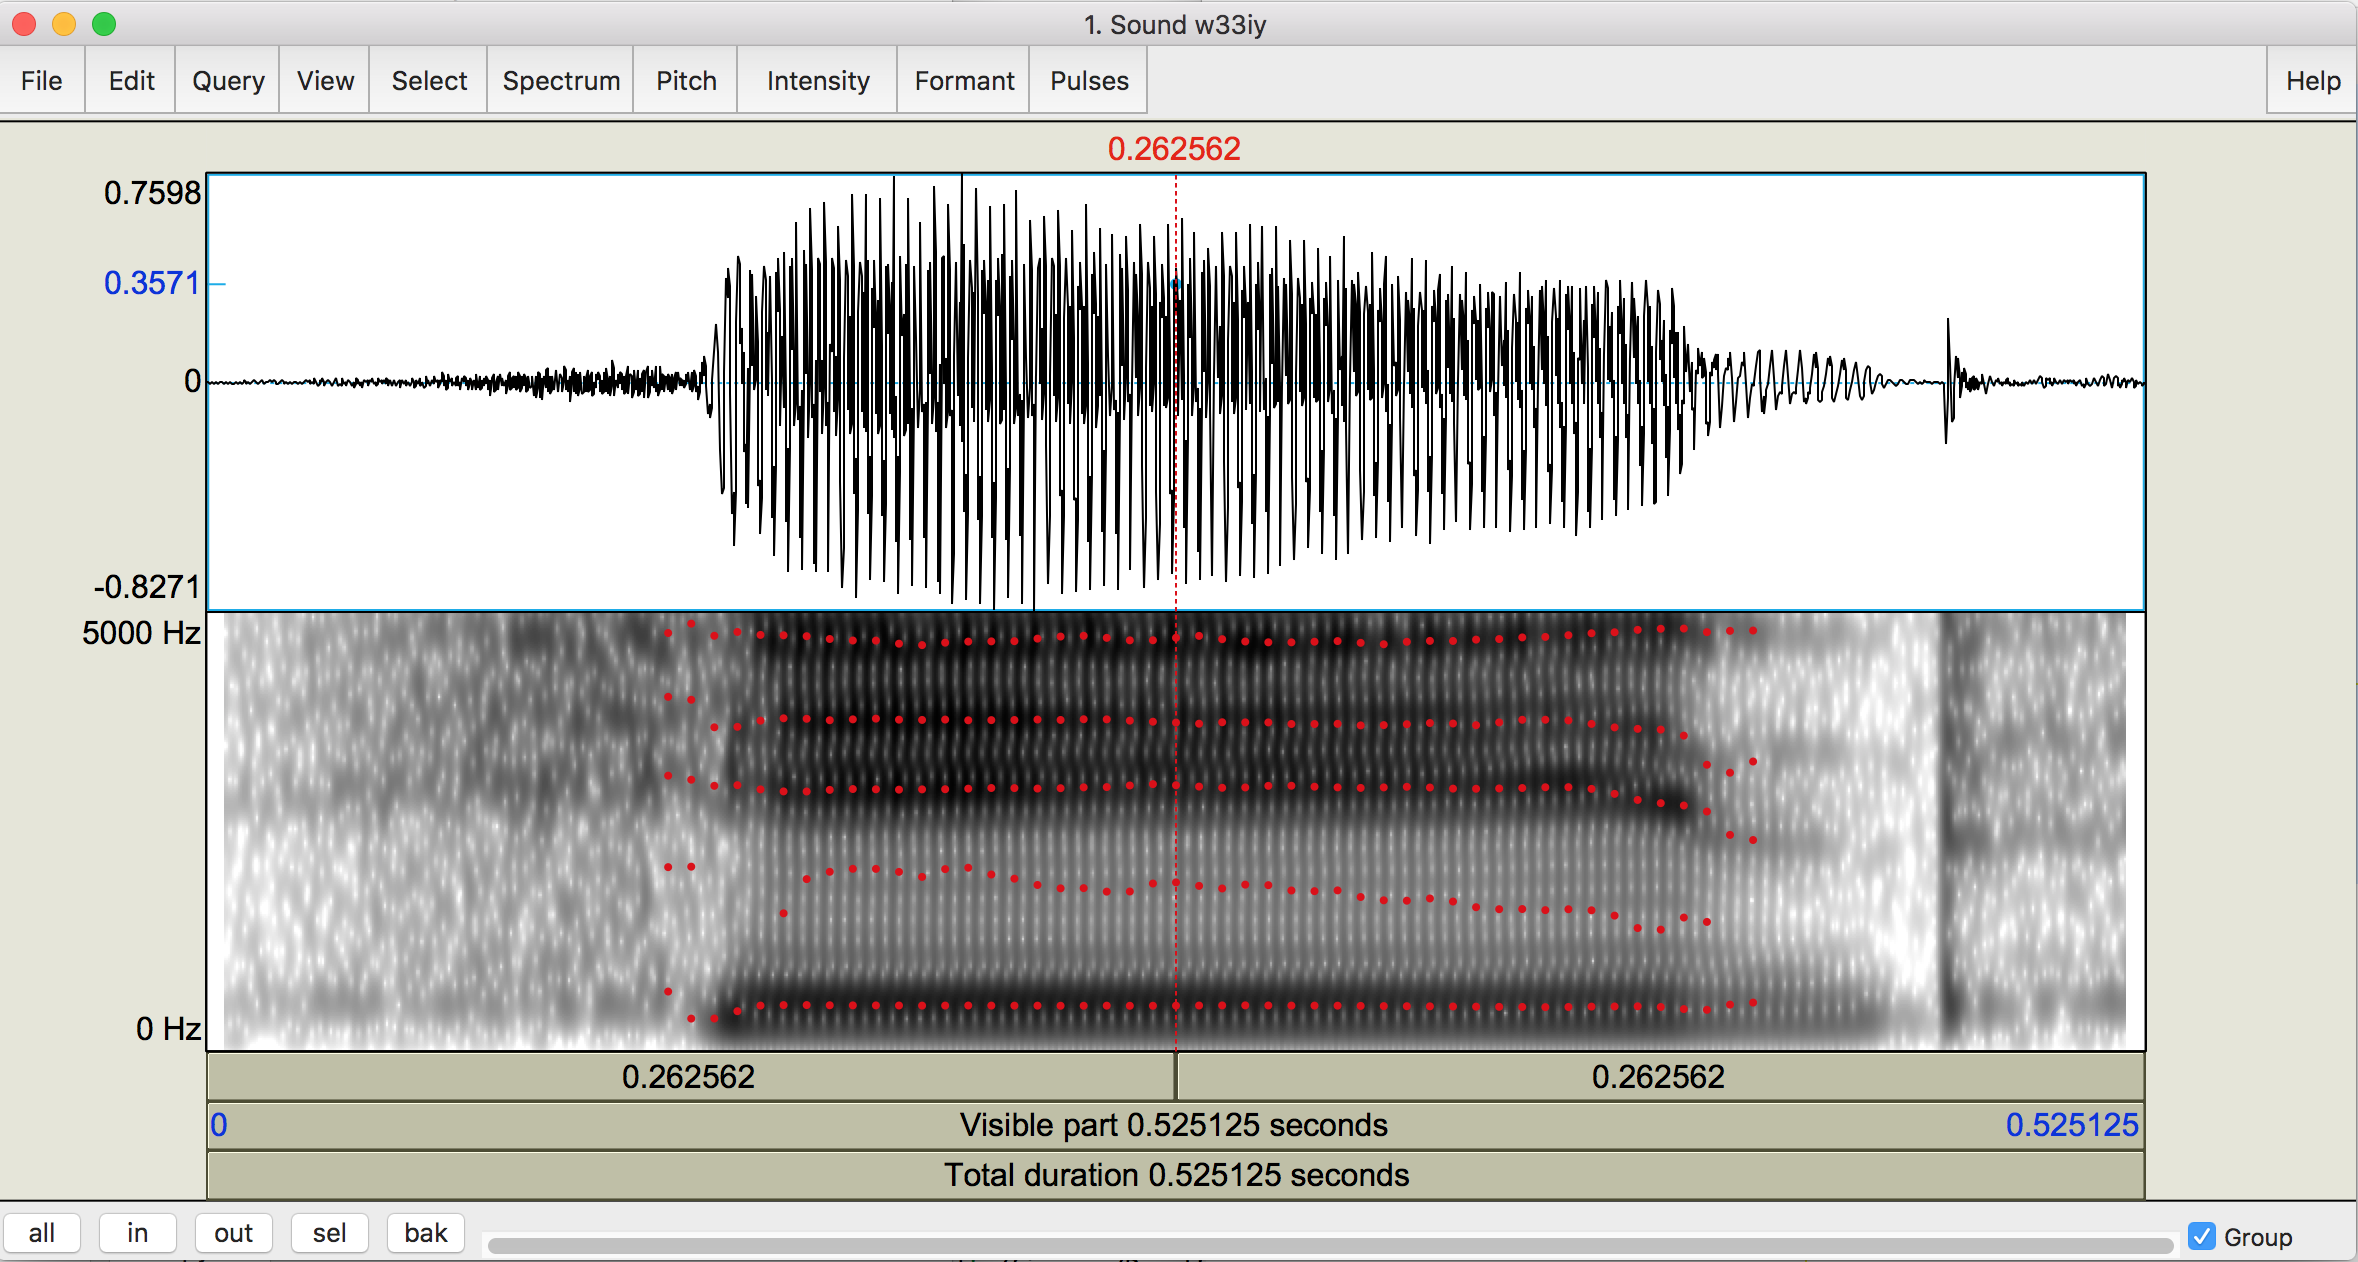
\includegraphics[width=0.8\textwidth]{./figures/Praat-05-View-and-edit}
	\end{center}
\end{figure}

The sound editor window displays the waveform (oscillogram) of the sound on the top part of the display and its spectrogram (figure~\ref{praat-view-and-edit}) immediately below it. You can play the sound by pressing the \softmenu{Total Duration} button at the bottom of the window. If you select a subpart of the sound by clicking and dragging the cursor over a portion of the waveform/spectrogram, a small pane with the duration of the selection will appear at both the top and bottom of the display; pressing either will play just the selected part of the sound, as shown in figure~\ref{praat-select-part-of-sound}.

\begin{figure}[!tbp]
\caption{\Praat{} -- View and Edit Window: Selection of part of the waveform for inspection}
\label{praat-select-part-of-sound}
	\begin{center}
		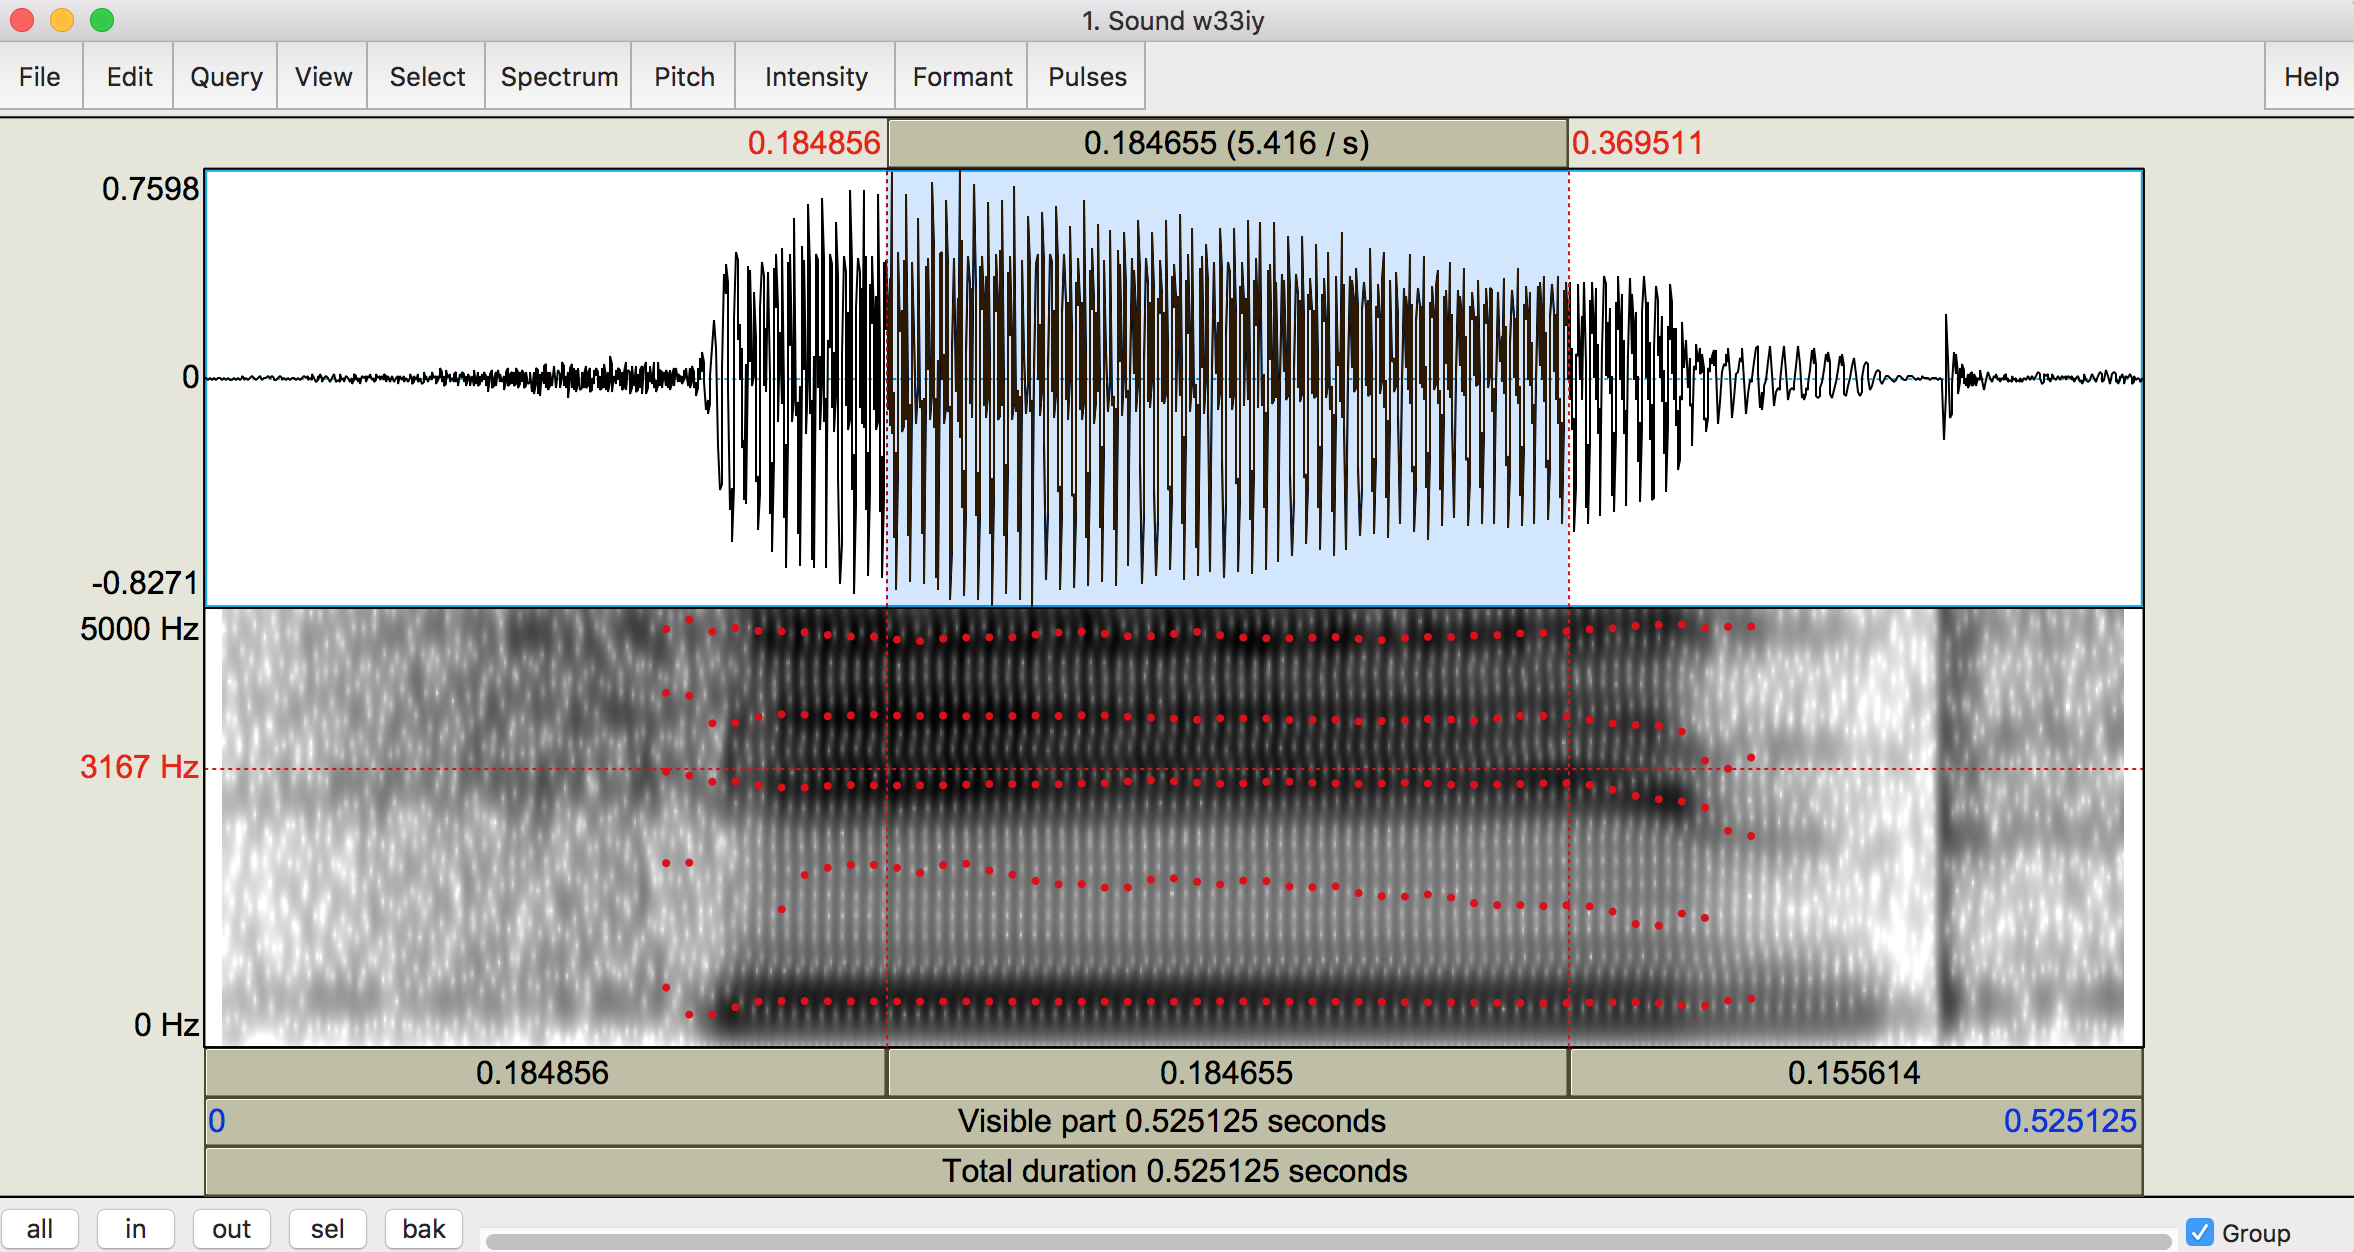
\includegraphics[width=0.8\textwidth]{./figures/Praat-06-Select-portion-of-sound}
	\end{center}
\end{figure}



\paragraph{Making the measurements.} Once you have your spectrogram in front of you, \Praat{} defaults to showing a series of red dots overlaid over the spectrogram. This is \Praat{}'s automatic formant tracking algorithm doing the best it can to display where the formants are for you. In case you don't see the red dots right away (or in case you inadvertently deselect the option of displaying them), you can turn it back on by going to \softmenu{Formant} $>$ \softmenu{Show Formants}. As you can see, \Praat{}'s formant tracking algorithm is pretty neat, but it is not flawless so make sure that the dots make sense given the underlying spectrogram.

If \Praat{} gave you reasonable formant tracks, then you can select a window over the center of the vowel -- its \emph{steady state} -- as shown in figure~\ref{praat-select-steady-state}, and go to \softmenu{Formant} $>$ \softmenu{Get first formant} (figure~\ref{praat-get-F1}). This should give you a window with a value, as shown in figure~\ref{praat-mean-F1}. Pay close attention to what that value represents (its unit of measurement, and whether it is a single or average measurement).

\begin{figure}[!tbp]
\caption{\Praat{} -- Getting the Formants automatically -- Selecting the \emph{steady state} of the vowel}
\label{praat-select-steady-state}
	\begin{center}
		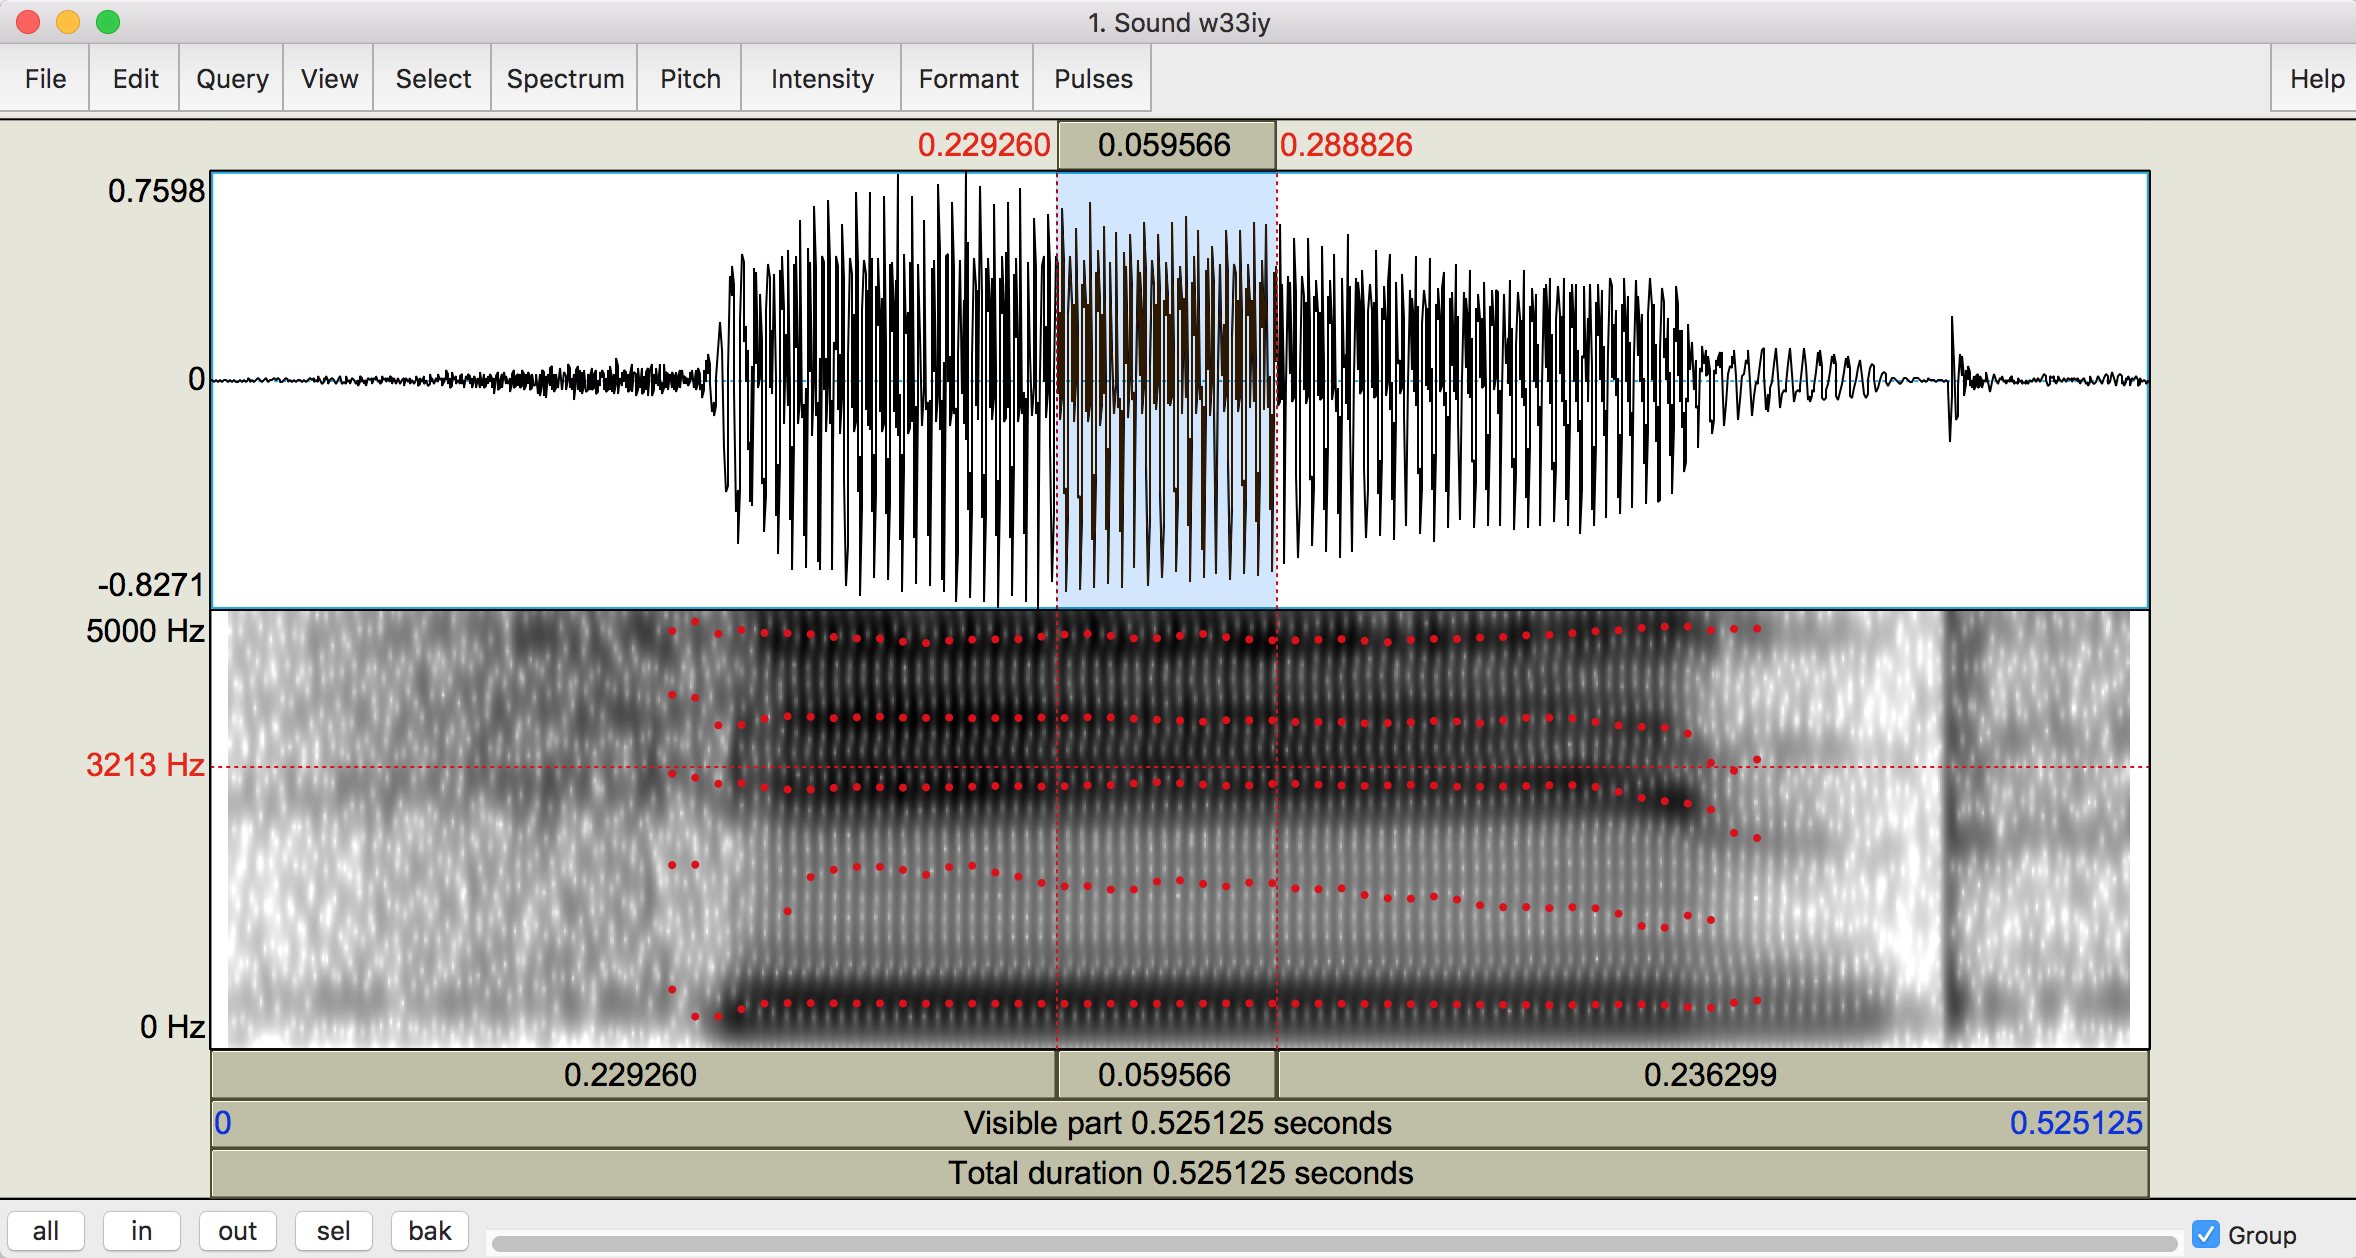
\includegraphics[width=0.8\textwidth]{./figures/Praat-07-Select-steady-state-vowel}
	\end{center}
\end{figure}

\begin{figure}[!tbp]
\caption{\Praat{} -- Getting the Formants automatically -- Automatically calculate F1}
\label{praat-get-F1}
	\begin{center}
		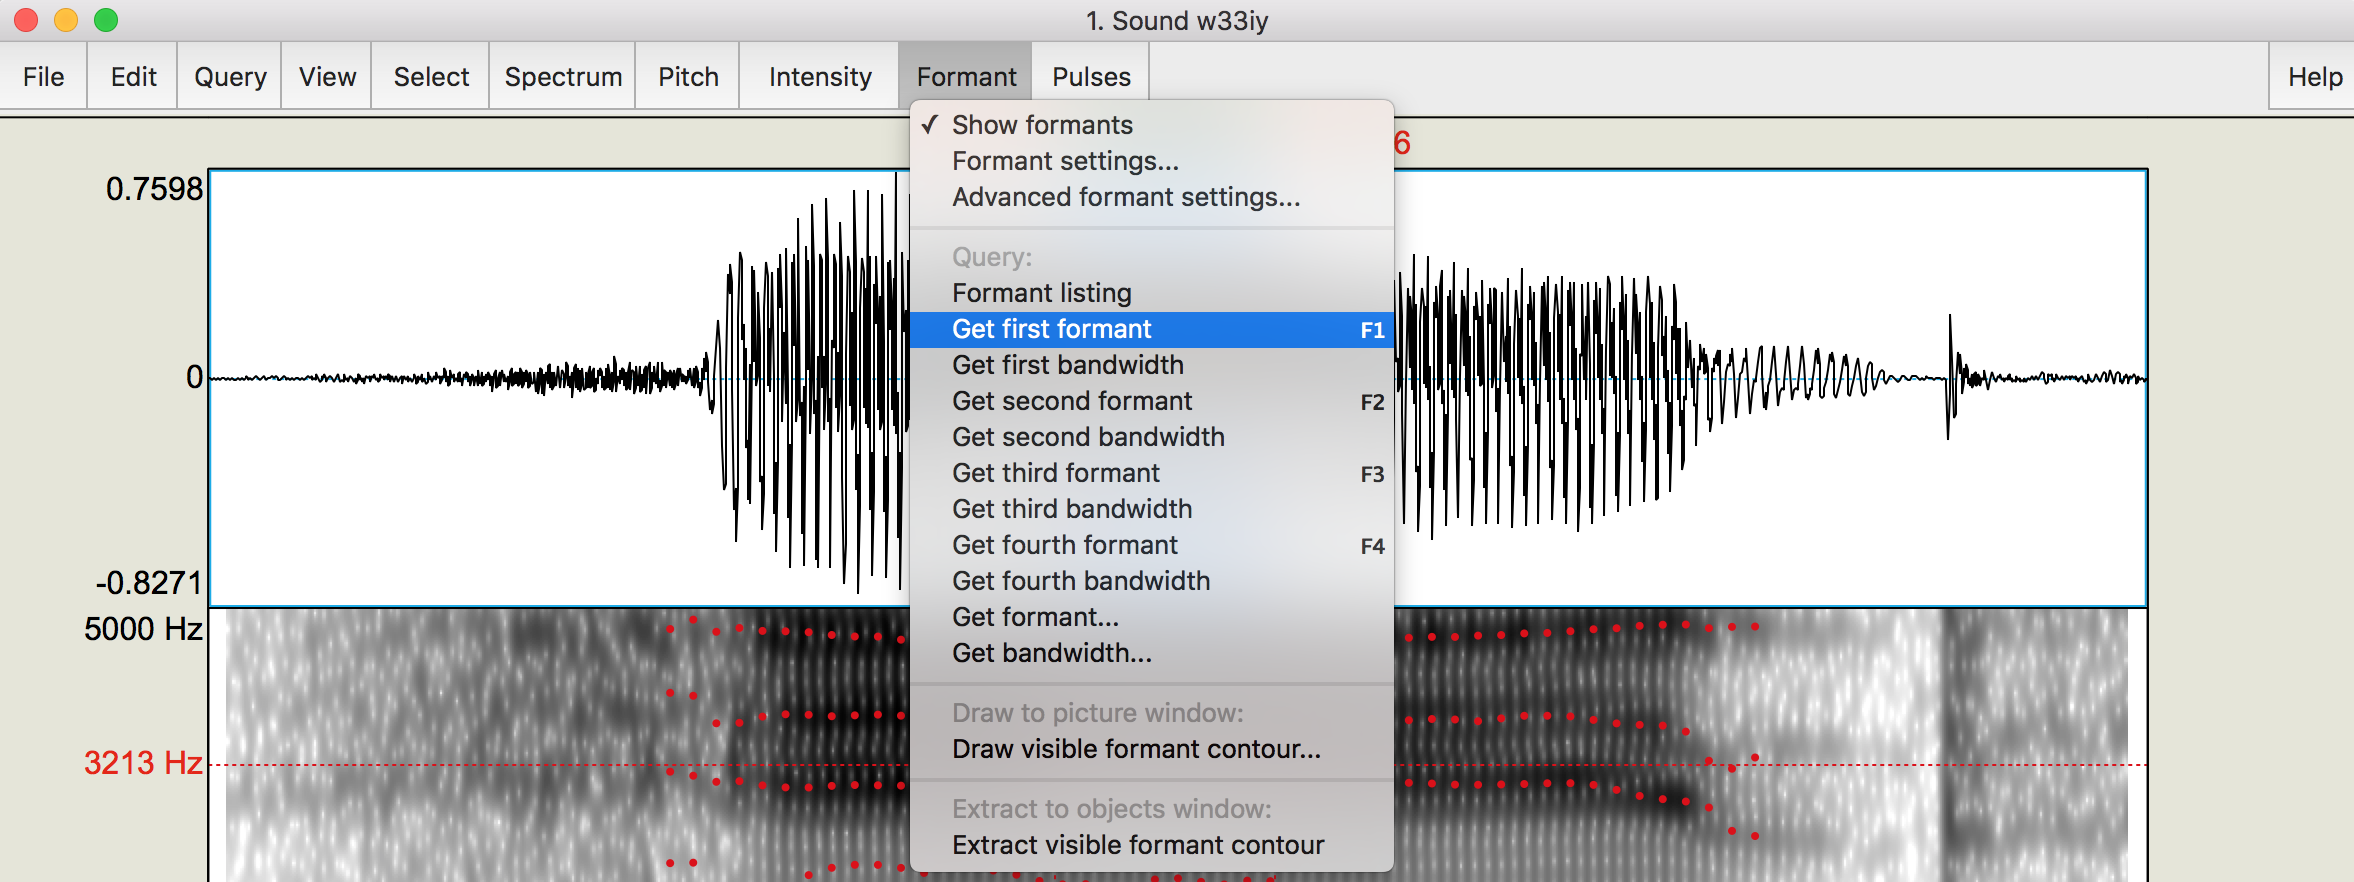
\includegraphics[width=0.8\textwidth]{./figures/Praat-08-Get-F1-from-selection}
	\end{center}
\end{figure}

\begin{figure}[!tbp]
\caption{\Praat{} -- Getting the Formants automatically -- Getting the mean F1 value over the vowel's \emph{steady state}}
\label{praat-mean-F1}
	\begin{center}
		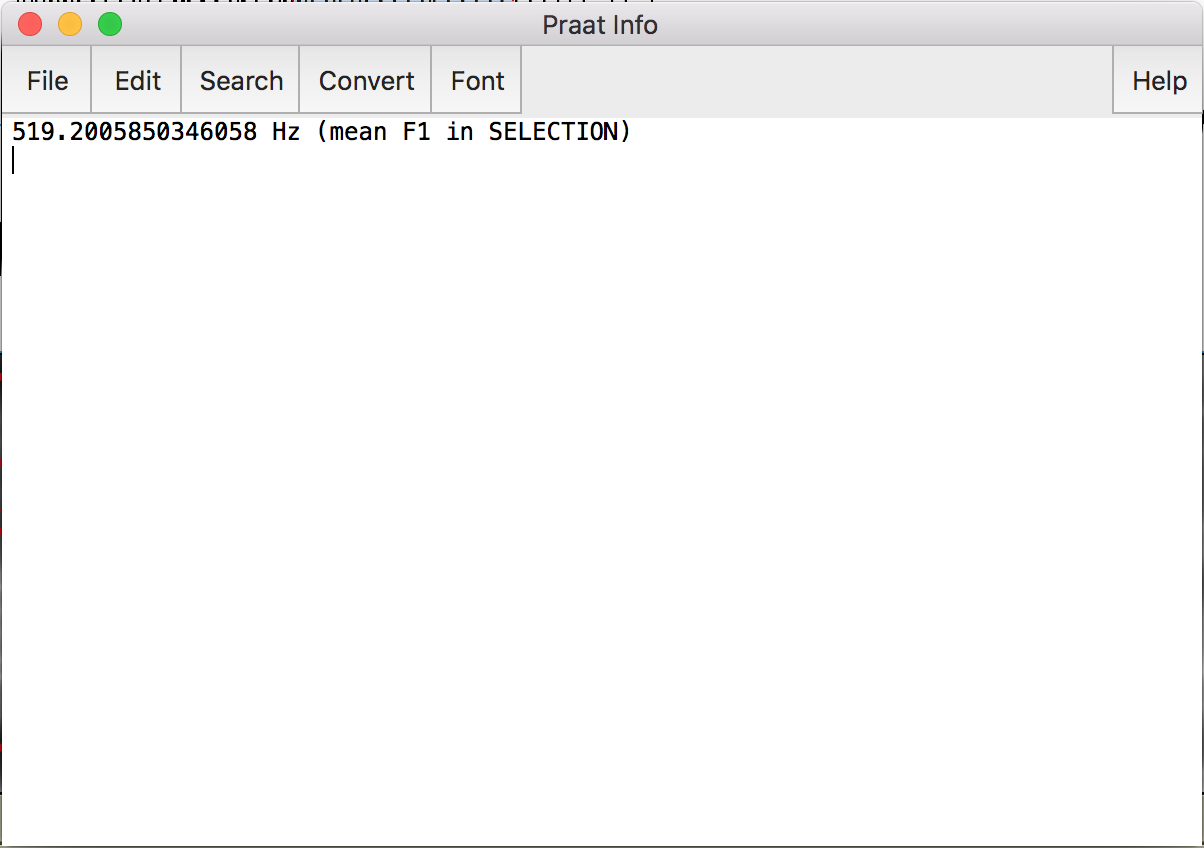
\includegraphics[width=0.8\textwidth]{./figures/Praat-09-Praat-info-window-F1}
	\end{center}
\end{figure}

If \Praat{} gave you formant tracks that don't seem to capture the formants you see adequately, then you can try to pin a couple of points in the formants (if you can easily see them on the spectrogram, which you should), get their values, average them and record that value in the spreadsheet. To get the value of any particular point, you can just click on it and \Praat{} will give you its value on the left side of the spectrogram in red. You can then jot down the numbers somewhere. If you want numbers that you can copy and paste, just click on the point, and then go to \softmenu{Spectrum} $>$ \softmenu{Get frequency at cursor}.

If you decide to do that, then you should be consistent across measurements. Choose the same number of points and be explicit about why you decided to take them. Finally, remember to follow the same procedures you used when measuring F1 when you measure F2.

\paragraph{Saving Formant values to a spreadsheet.} Once you get your formant values, you should start saving them into a spreadsheet. Remember to label the values appropriately, as shown in figure~\ref{saving-f1-f2}.

\begin{figure}[!tbp]
\caption{\MSExcel{} -- Saving the Formant values of each recording}
\label{saving-f1-f2}
	\begin{center}
		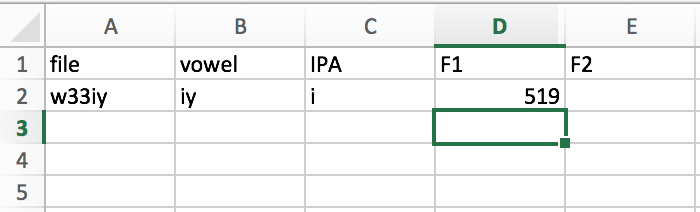
\includegraphics[width=0.8\textwidth]{./figures/SavingF1F2-10-Spreadsheet}
	\end{center}
\end{figure}

Once you finish copying the values to the spreadsheet, you should export them to a \emph{comma separated value} file or \filefmat{csv} file, so that you can then import the values to \Praat{} for plotting. Every spreadsheet program should have an \softmenu{export} or \softmenu{save as} option that allows you to save the contents in a worksheet to a \filefmat{csv} file.

\paragraph{CSV.} The \emph{comma separated file} is a pure text format used to represent tabular data, the kind that is normally inspected and manipulated by spreadsheet programs. However, unlike the binary formats used by these programs, \filefmat{csv} files can be opened by any text editor and is a useful format for transferring data across different pieces of software.

\paragraph{IPA symbols for the vowels.} In order to plot the values you measured from a particular individual, you need to save not only the vowel codes used by \citeA{hillenbrand1995}, but the actual IPA symbols will look better in a graph. Here's how you should input the IPA symbols in your spreadsheet in order to plot them appropriately in \Praat{}:

\begin{enumerate}
\item \filefmat{w33iy.wav}: i = i
\item \filefmat{w33ih.wav}: \textsci{} = \textbackslash{}ic
\item \filefmat{w33eh.wav}: \textepsilon{} = \textbackslash{}ef
\item \filefmat{w33ae.wav}: \ae{} = \textbackslash{}ae
\item \filefmat{w33ah.wav}: \textscripta = \textbackslash{}as
\item \filefmat{w33aw.wav}: \textopeno = \textbackslash{}ct
\item \filefmat{w33uh.wav}: \textupsilon{} = \textbackslash{}hs
\item \filefmat{w33uw.wav}: u = u
\end{enumerate}

\paragraph{Example \filefmat{csv} file.} I created a small example of what the \filefmat{csv} should look like. It is named \emph{american-vowels-example.csv}. This file is distributed with the rest of the lab resources, and it contains the measurements of F1 and F2 for just three vowels ([i], [\textscripta] and [u]) for the \emph{w33} participant.

\subsubsection{Plotting the Formant values}

\paragraph{Using the plot functions of \Praat{}.} There are many ways in which you could plot your measurements. Any decent spreadsheet program would allow you to create a simple scatterplot. Unfortunately, how you can accomplish this task will vary not only across programs, but also within different versions of the same program (an older version of this lab from 2013 became largely obsolete because of software changes in \MSExcel{}, for instance). Ideally, one should use a real programming language with good plotting capabilities, like \soft{R} or \soft{Python}. The downside is that the learning curve can be a little steep in case you never did any programming. Since the goal of this lab is to get you to interpret phonetic data graphically without getting too bogged down in general implementation details, I eventually settled on using \Praat{} to plot the data. It's a bit of an \emph{ad-hoc} solution --- I would not recommend that you use \Praat{} as your plotting solution for other kinds of data --- but it works quite well for the kind of data we have at hand, and it produces publication--ready figures with minimal fuss.

\paragraph{Inspecting your data.} Once you have the the average formant values, you are ready to plot your data. The first step is to read your measurements into \Praat{}. In the \softmenu{Praat Objects} window, click on \softmenu{Open} and then on \softmenu{Read Table from comma separated file}, as shown in figure~\ref{praat-read-table-csv}.

\begin{figure}[!tbp]
\caption{\Praat{} -- Read your data from \emph{comma separated value} file}
\label{praat-read-table-csv}
	\begin{center}
		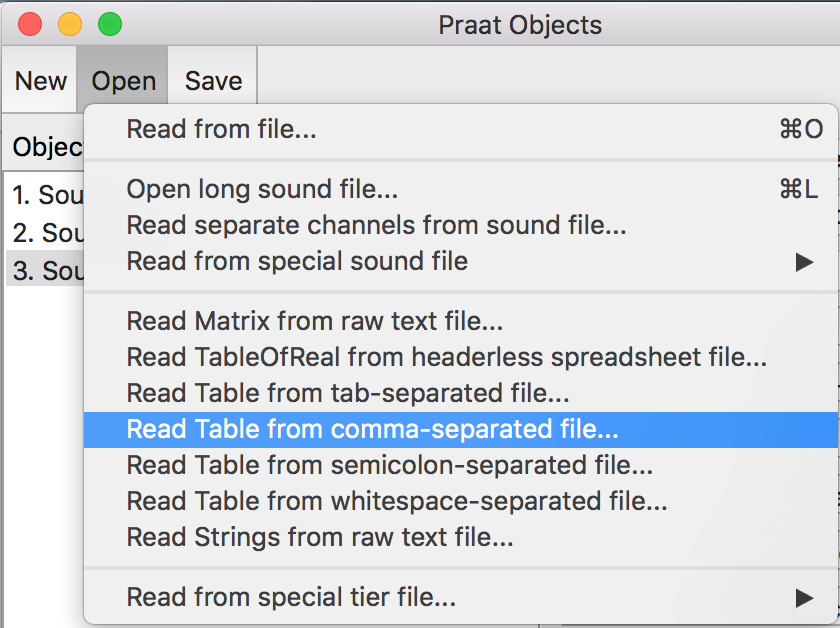
\includegraphics[width=0.8\textwidth]{./figures/Praat-11-Read-Table}
	\end{center}
\end{figure}

The command \softmenu{Read Table from comma separated file} takes a \filefmat{csv} file and produces a \emph{Table} object in \Praat{}, as shown in figure~\ref{praat-table-in-objects}. A \emph{Table} object in \Praat{} can organize tabular data, much like a spreadsheet. You can inspect its contents by pressing the button \softmenu{View \& Edit} after you select (click on) the object in the \softmenu{Praat Objects} window, as shown in figure~\ref{praat-inspect-table}. However, unlike in a real spreadsheet program, a \Praat{} \emph{Table} object cannot be directly modified by clicking and typing, it can only be modified via cumbersome menu options. Thus, if you notice something wrong with the \filefmat{csv} file you just imported when you inspect it in \Praat{}, I strongly suggest that you open it on a spreadsheet program and edit there, and then try to read it in again into \Praat{}.

\begin{figure}[!tbp]
\caption{\Praat{} -- Newly created \emph{Table} object in the \softmenu{Objects} window}
\label{praat-table-in-objects}
	\begin{center}
		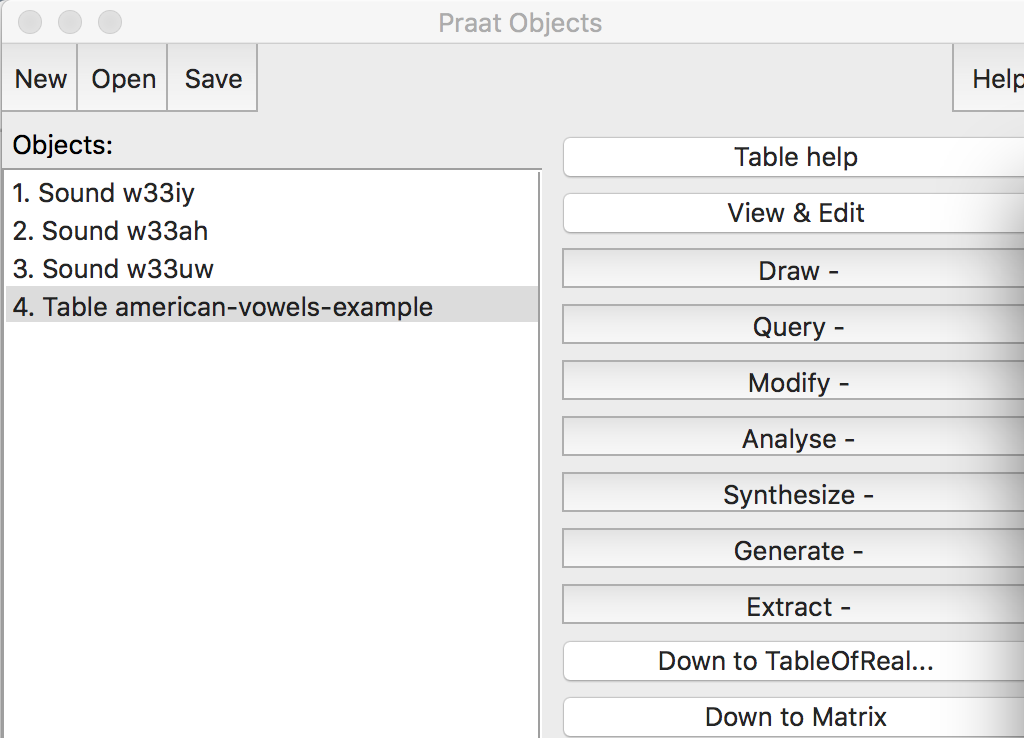
\includegraphics[width=0.8\textwidth]{./figures/Praat-12-Table-object-in-window}
	\end{center}
\end{figure}


\begin{figure}[!tbp]
\caption{\Praat{} -- Visually inspecting Table object}
\label{praat-inspect-table}
	\begin{center}
		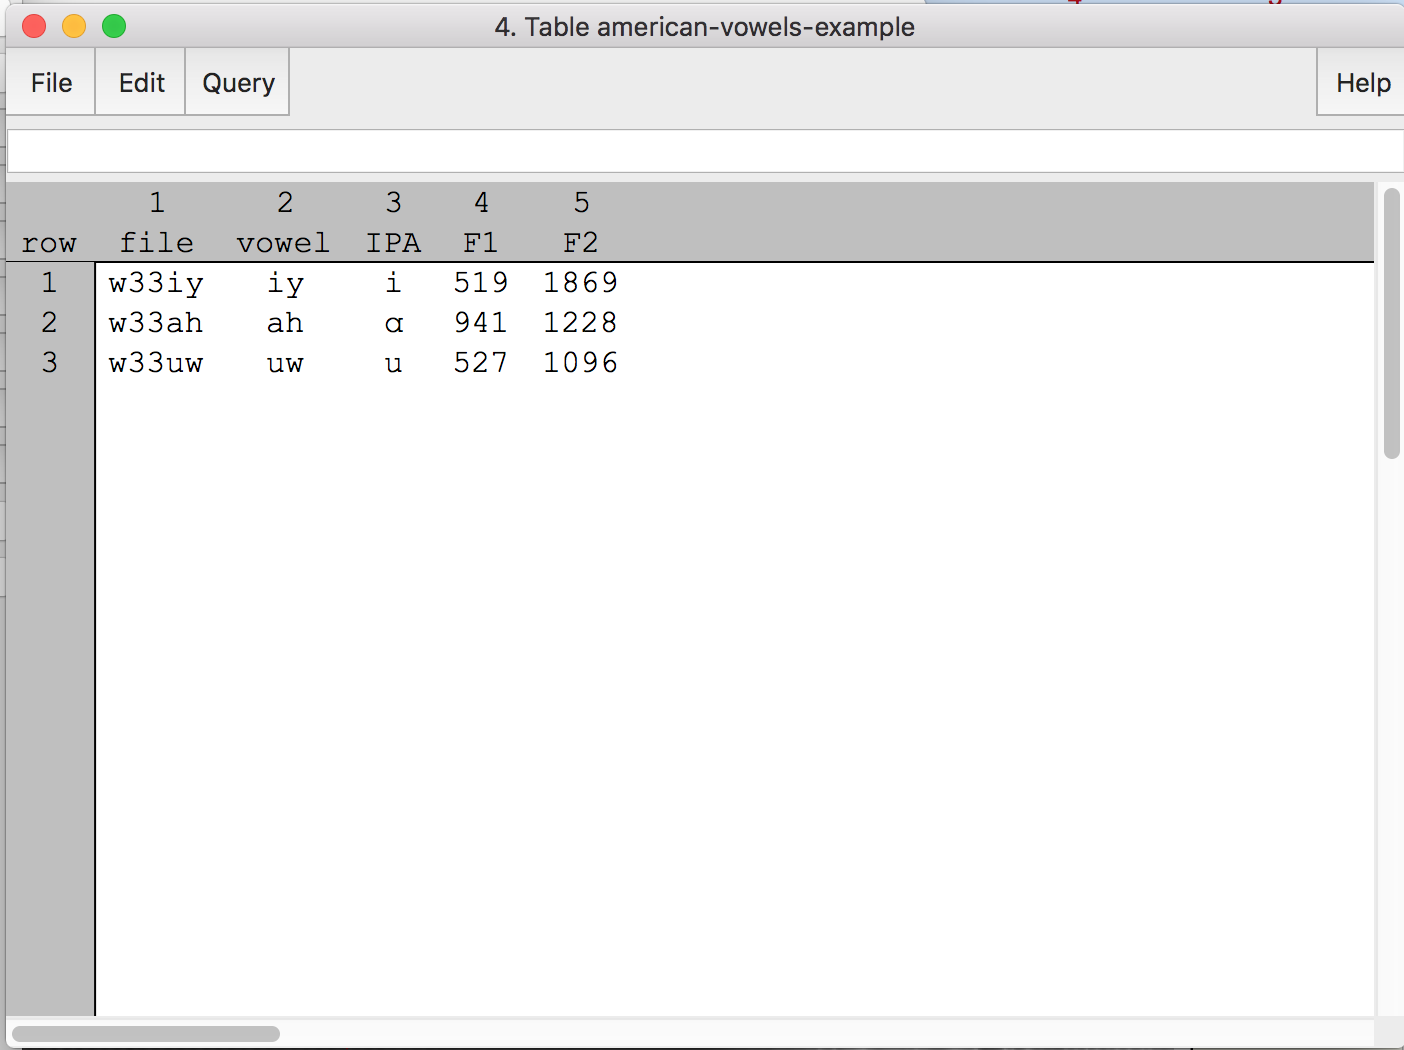
\includegraphics[width=0.8\textwidth]{./figures/Praat-13-Table-inspect}
	\end{center}
\end{figure}

\paragraph{Plotting your data.} Once you are satisfied that your data has been collected appropriately and read into \Praat{} correctly, you can create a scatterplot for the F1 and F2 values that you measured. Click on \softmenu{Draw} $>$ \softmenu{Scatter plot}, as shown in figure~\ref{praat-scatterplot-vowels}. This will bring up a dialog window asking you which variable (i.e., column) of your table object should be plotted on the horizontal (i.e, x--axis) and the vertical (i.e., y--axis), as well as the range of each axis. It also asks which variable (i.e., column) contains the symbols that are going to be used for plotting in the \softmenu{Column with marks} textbox, the font size to use, and finally whether you want to plot all the axes information and a box around the plot (the \softmenu{Garnish} checkbox option).

\begin{figure}[!tbp]
\caption{\Praat{} -- Visually inspecting Table object}
\label{praat-scatterplot-vowels}
	\begin{center}
		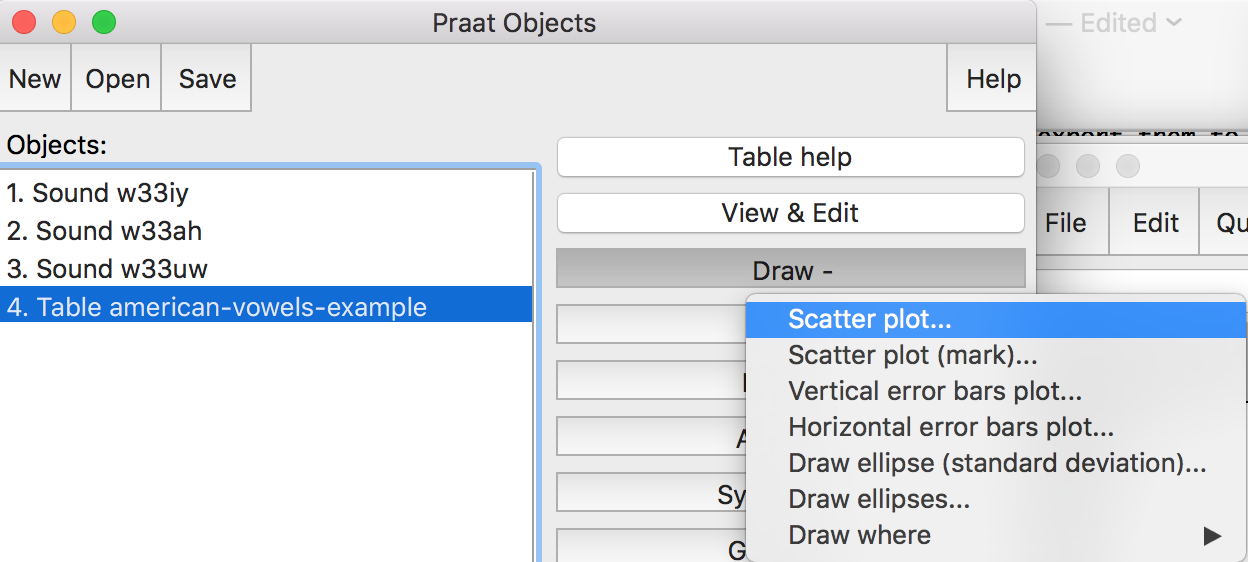
\includegraphics[width=0.8\textwidth]{./figures/Praat-14-Scatterplot-01}
	\end{center}
\end{figure}

You should fill out this dialog box such that F2 is displayed on your x--axis, F1 in your y--axis, and that the column containing the IPA symbols for the vowels you measured (I suggest you use the name IPA for that column, for obvious reasons) is used in the \softmenu{Column with marks} textbox. Finally, the default fontsize 12 is ok, and you should plot all the axis information, so make sure that the \softmenu{Garnish} checkbox is checked.

\paragraph{A note on the range of the axes.} Even though \Praat{} offers you to set the ranges of your axes automatically, here you should avoid that, because we will want to produce overlaid plots (i.e., plots on top of other plots). Therefore, you should you use a preset set of values for the range of your axes such that your plot will be able to accommodate as many plausible vowel values as possible. I suggest that you use the values below.

\begin{description}
\item[minimum value for F1] 150
\item[maximum value for F1] 1300
\item[minimum value for F2] 500
\item[maximum value for F2] 3300
\end{description}

%% min F1 for women = 220 --> use 150
%% max F1 for women = 1110 --> use 1200
%% min F2 for women = 590 ---> use 500
%% max F2 for women = 3100 ---> use 3200

%% min F1 for men = 190 --> use 150
%% max F1 for men = 860 --> use 1200
%% min F2 for men = 560 --> use 500
%% max F2 for men = 2700 --> use 3000

%% min F1 in whole PB data = 190
%% max F1 in whole PB data = 1300
%% min F2 in whole PB data = 560
%% max F2 in whole PB data = 3610

Another important piece of information is that each axis has two boxes where you can establish its range. For the x--axis, the left box indicates the limit on the left side of the plot and the right box the limit on the right side of the plot. Likewise, on the y--axis, the left box indicates the limit on the bottom side of the plot and the right box the limit on the top side of the plot. Thus, if you want your plot to have increasing values from left-to-right and bottom-to-top, you should input the lower bound of each axis on the left boxes and the upper bounds on the right boxes. If you wanted to plot axes that presented information in the opposite pattern, all you would need to do is invert the values you use for the left and right bounds. Figure~\ref{praat-scatterplot-dialog} indicates how you should initially fill the dialog box for the plot, and figure~\ref{praat-scatterplot-result} shows the result for the example data I've provided (only for three vowels, you should have more vowels in your plot).

\begin{figure}[!tbp]
\caption{\Praat{} -- Scatterplot dialog box}
\label{praat-scatterplot-dialog}
	\begin{center}
		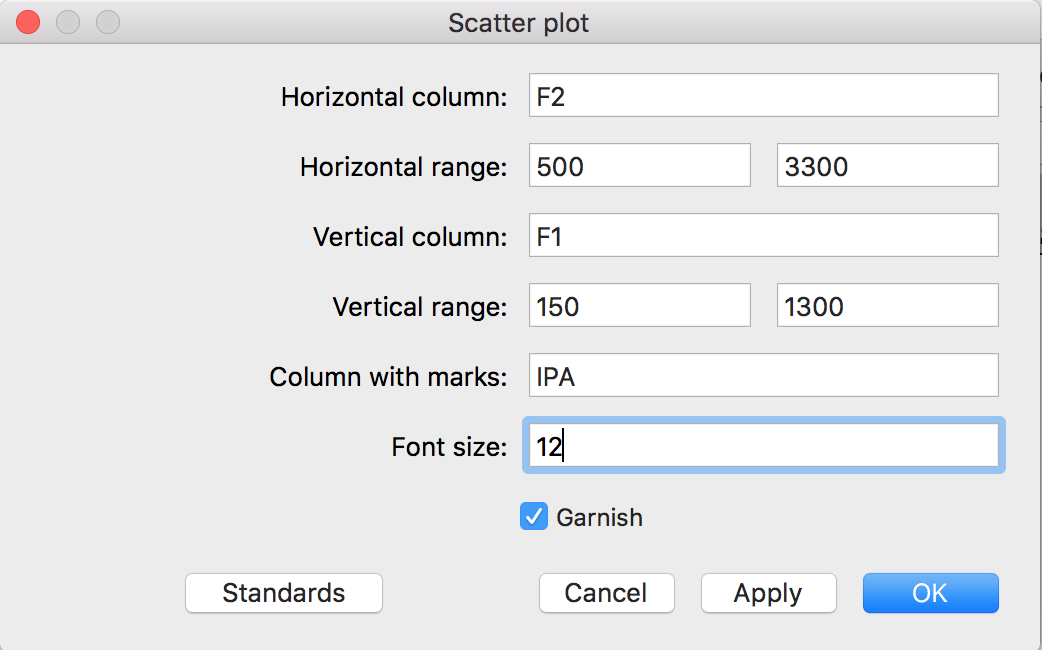
\includegraphics[width=0.8\textwidth]{./figures/Praat-15-Scatterplot-02}
	\end{center}
\end{figure}

\begin{figure}[!tbp]
\caption{\Praat{} -- Scatterplot result}
\label{praat-scatterplot-result}
	\begin{center}
		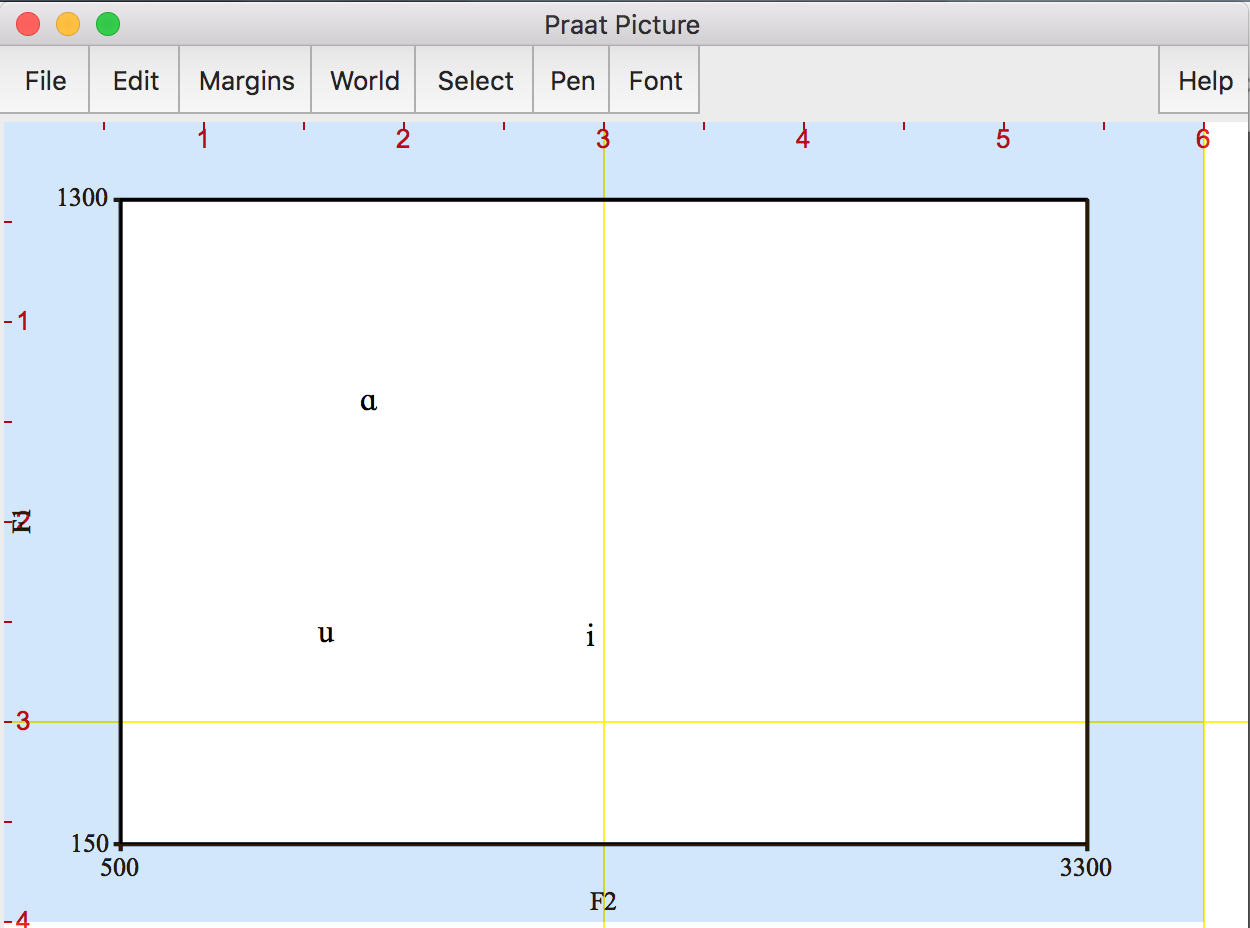
\includegraphics[width=0.8\textwidth]{./figures/Praat-16-Scatterplot-Output}
	\end{center}
\end{figure}

\paragraph{Saving your graph.} You can save your graph by clicking on \softmenu{File} on the \softmenu{Praat Picture} window and selecting the most appropriate format. I strongly suggest either \filefmat{.pdf} or \filefmat{.png}, as they are easy to embed in most modern text processing applications.

\paragraph{Interpreting the graph.} Plotting a graph is not just about being able to see data, but rather being able to see data \emph{in the most informative way} possible. So you should ask yourself certain questions like \emph{Do I need a legend if the points are labeled?}, \emph{Does the range of the scale on the axes make sense?}, and so on. Creating a good graph necessitates thinking in some detail about what relevant features of your data you want to convey. This will turn out to be important in the future, so keep that in mind.

In this case, the basic plot parameters were given by me, but in the future when you start producing your own graphs, you will need to really think about how to best convey the information you want to convey in a graph. For instance, take a look at the graph of the F1 and F2 values you just created. Does it suggest any pattern to you? (hint: think back to your IPA chart). If so, is the way the graph is currently set up the best way to see this pattern? If not, how should you modify your plot in order to make the relevant pattern more immediately accessible to the reader/viewer? Try to produce this plot and see if the pattern becomes clearer. You can always erase a particular graph from your current \softmenu{Praat picture} window by clicking on \softmenu{Edit} $>$ \softmenu{Erase All}, as shown in figure~\ref{praat-erase-plots}.

\begin{figure}[!tbp]
\caption{\Praat{} -- Erasing plots from Picture window}
\label{praat-erase-plots}
	\begin{center}
		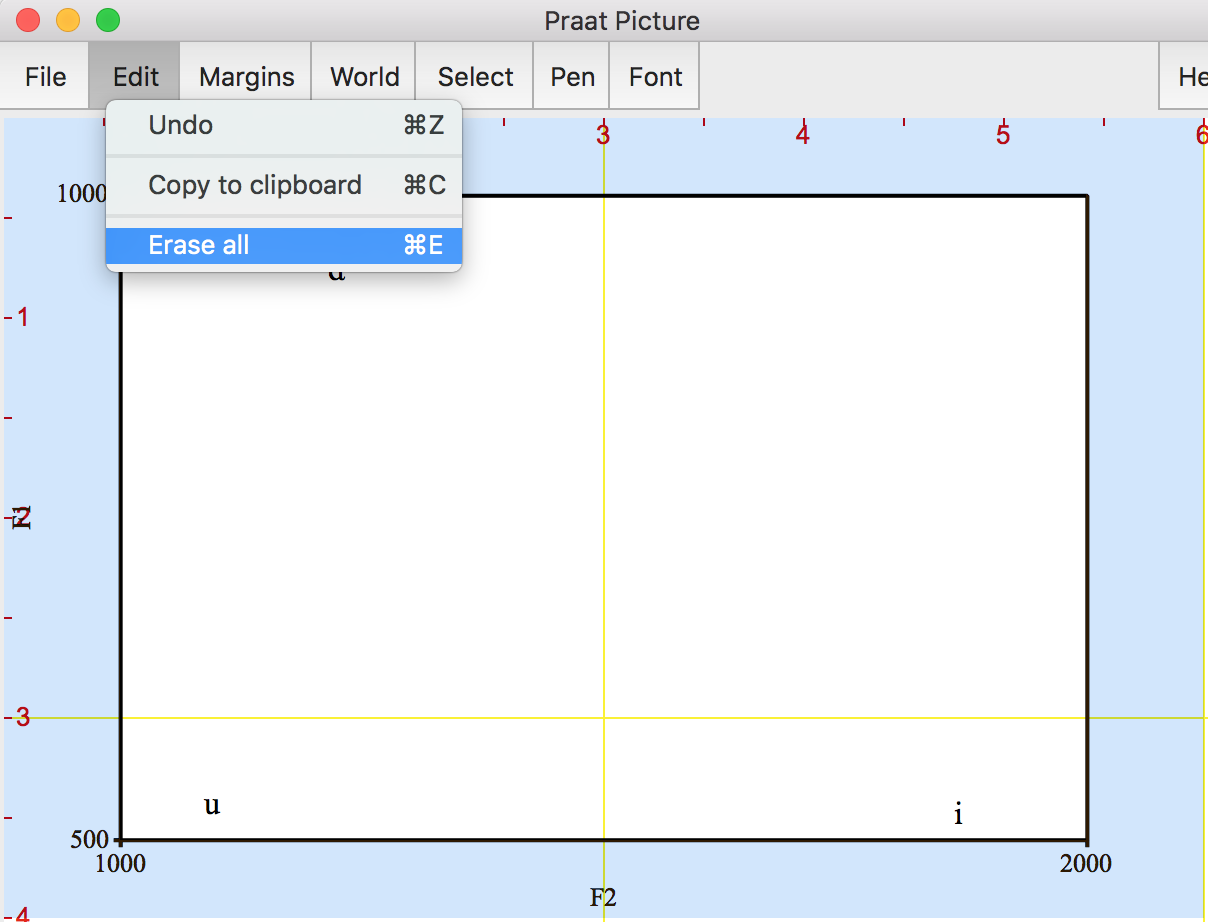
\includegraphics[width=0.8\textwidth]{./figures/Praat-Erase-Plots}
	\end{center}
\end{figure}

Another important aspect in the interpretation of a graph is what aspect of a particular research question it is supposed to shed light on. In the context of our class, there were two major questions we left unanswered:

\begin{enumerate}
\item How do the acoustic representations of speech relate to the articulatory ones?
\item Is there a one--to--one mapping function between simple features of acoustic representations and articulatory representations of speech?
\end{enumerate}

By now, you should be able to give at least a partial answer to question 1 above, given your data, especially if you were able to produce the most informative version of the plot we started to construct above. However, we can only give a very tentative kind of answer to question 2. This is because even if you were able to notice a one--to--one mapping between acoustic and articulatory features, we can only be certain that it holds for the particular individual you happened to have analyzed. In order to make a well--supported generalization, we would need data from more individuals and see whether the pattern you observed in one person holds across multiple individuals.

\paragraph{Putting the graph in context, part I.} By now, you should have observed that there is a particular link between features of the acoustic representation of vowels in terms of its spectrogram and their articulatory features. The question you need to answer is whether the pattern you observed in the individual holds in a larger population of speakers of the same dialect.

Fortunately for us, some people have already collected the relevant data for American English, and this data is already packaged as a \Praat{} \emph{Table} object. Go to \softmenu{New} $>$ \softmenu{Tables} $>$ \softmenu{Create formant table (Peterson and Barney 1952)}, as shown in figure~\ref{praat-pb-table}. This will load up a \emph{Table} object containing the measurements of F0, F1, F2 and F3 from \citeA{peterson1952} on 33 males, 28 women and 13 children. All we need to do is plot the F1 and F2 values from that database and we will have a clearer sense of whether your original observation holds for a larger population. At this point, you should have a \emph{Table} object \emph{pb} on your \softmenu{Objects} list (figure~\ref{praat-pb-table}). If you click on \softmenu{View \& Edit}, you can inspect it (see figure~\ref{praat-pb-table-inspection}).

\begin{figure}[!tbp]
\caption{\Praat{} -- Loading Peterson \& Barney 1952 data}
\label{praat-pb-table}
	\begin{center}
		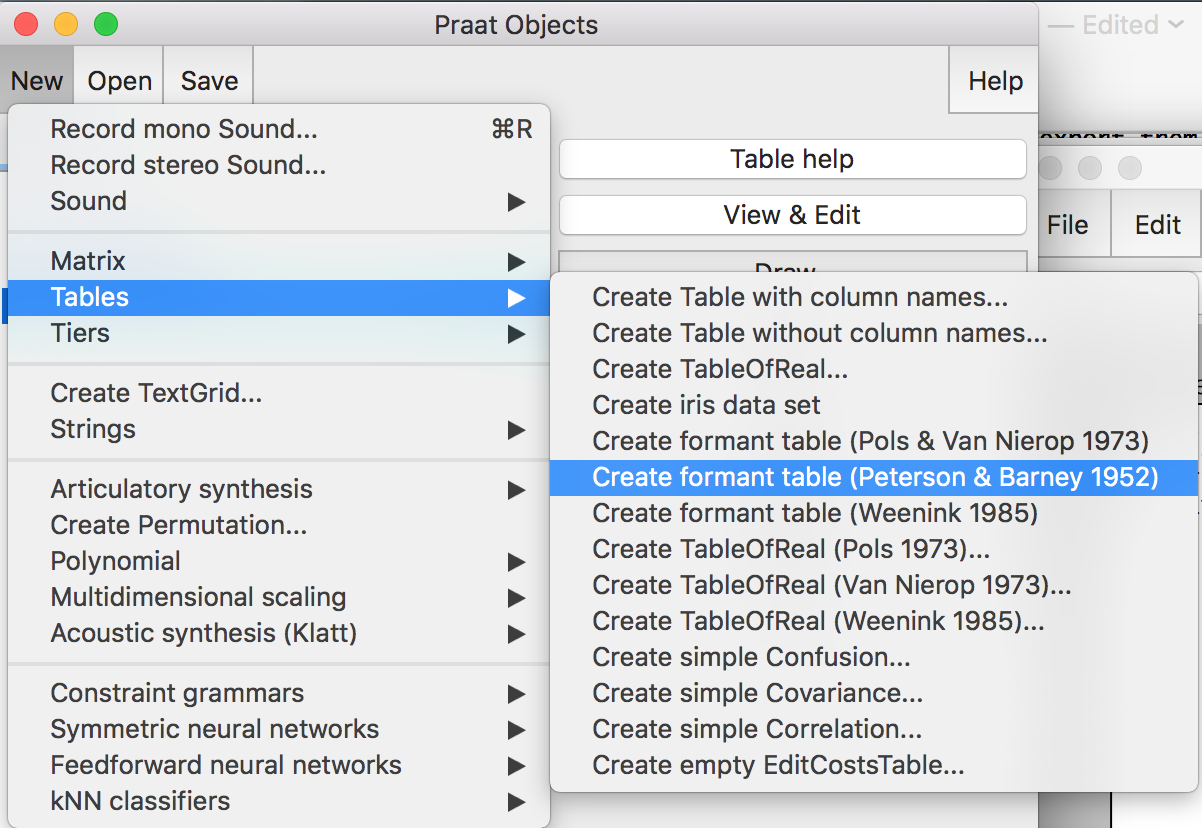
\includegraphics[width=0.45\textwidth]{./figures/Praat-17-PB-table}
		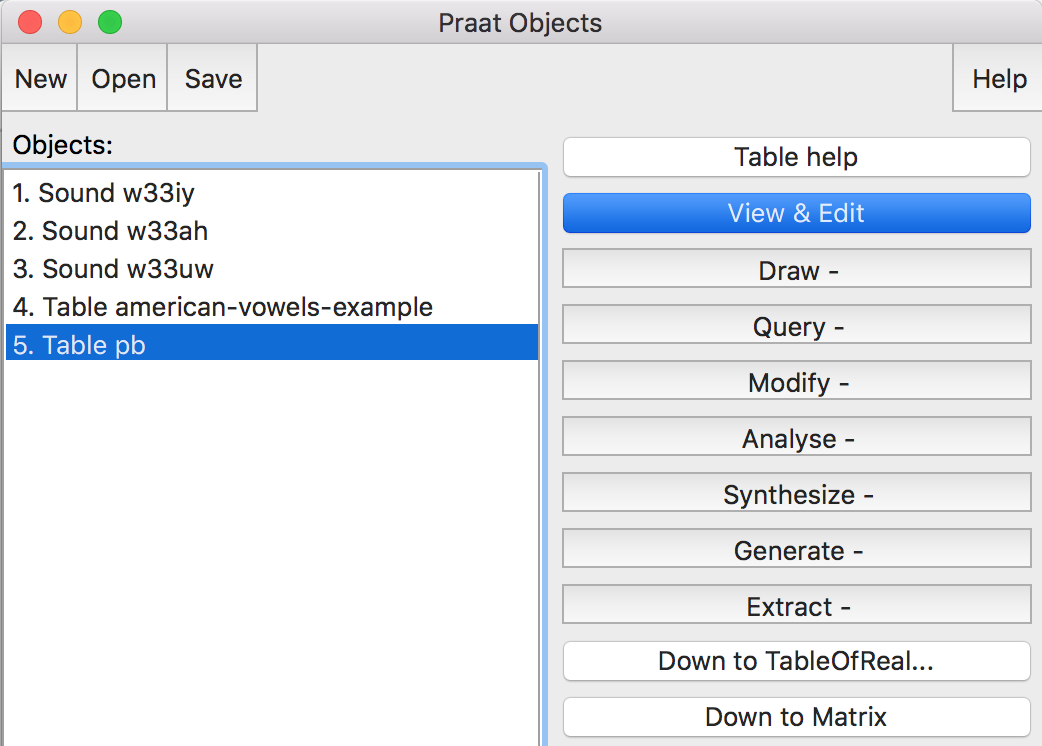
\includegraphics[width=0.45\textwidth]{./figures/Praat-18-PB-table-in-objects}
	\end{center}
\end{figure}


\begin{figure}[!tbp]
\caption{\Praat{} -- Inspecting Peterson \& Barney 1952 data}
\label{praat-pb-table-inspection}
	\begin{center}
		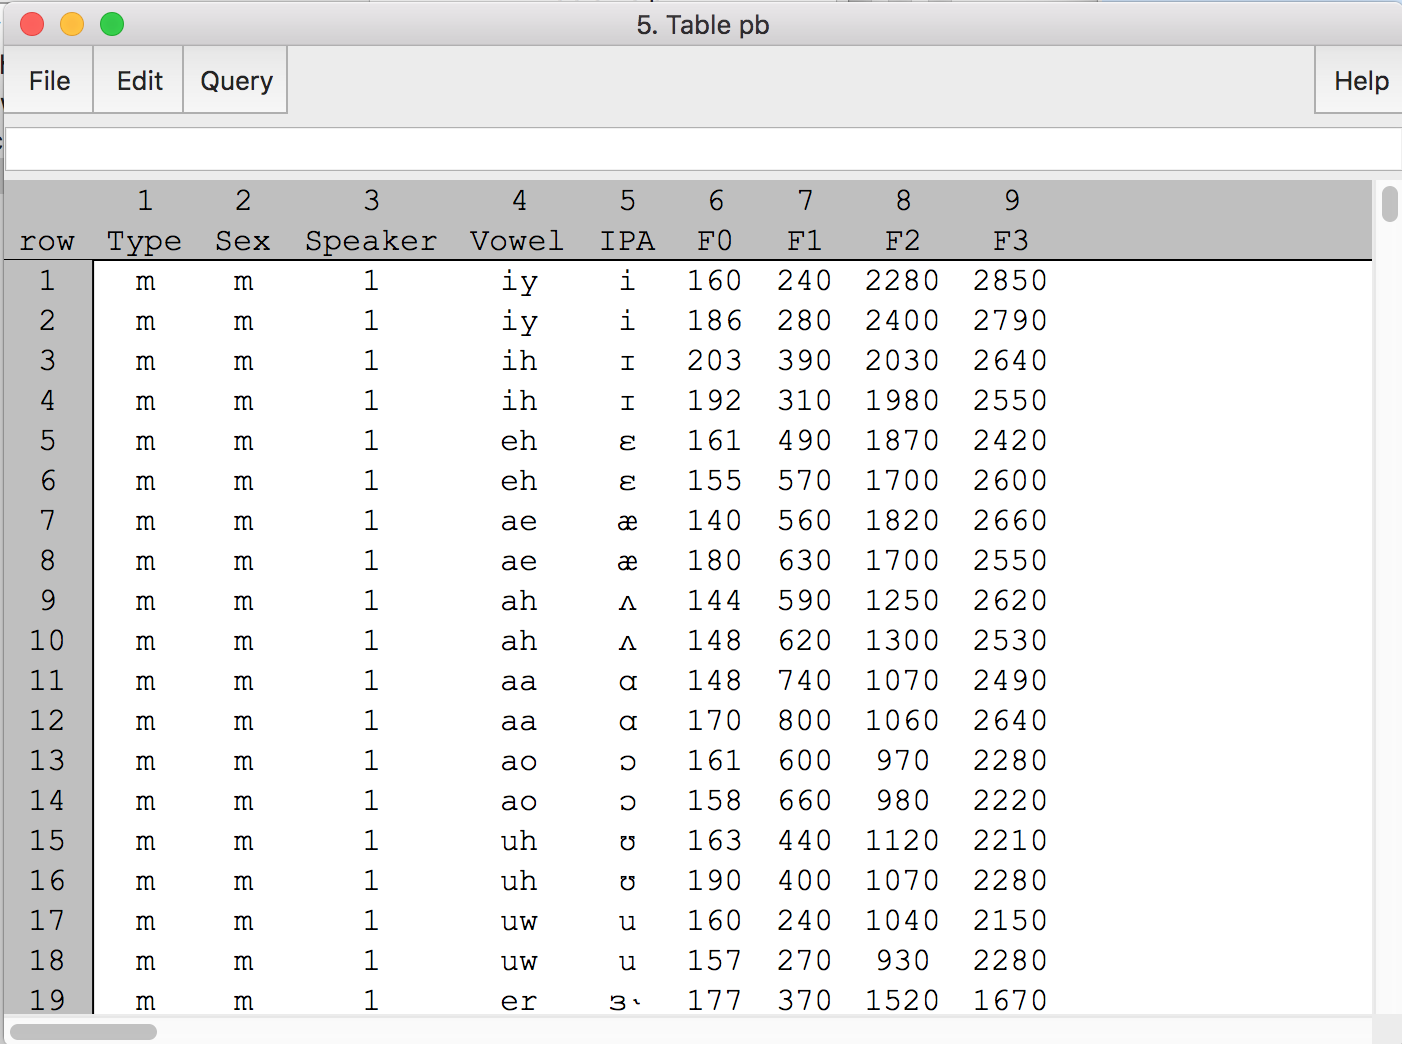
\includegraphics[width=0.8\textwidth]{./figures/Praat-19-PB-table-inspect}
	\end{center}
\end{figure}

Follow the next steps:

\begin{enumerate}
\item Make sure you are starting with a blank \softmenu{Pictures window}. If your \softmenu{Pictures window} has already a plot on it, just erase its current contents by clicking \softmenu{Edit} $>$ \softmenu{Erase all}.
%
\item Select the \emph{Table pb} on the \softmenu{Objects window}, then go to \softmenu{Extract} $>$ \softmenu{Extract rows where column (text)\ldots}, as in figure~\ref{praat-pb-table-extraction}.
%
\begin{figure}[!tbp]
\caption{\Praat{} -- Extracting subset of data in the Peterson \& Barney 1952 dataset}
\label{praat-pb-table-extraction}
	\begin{center}
		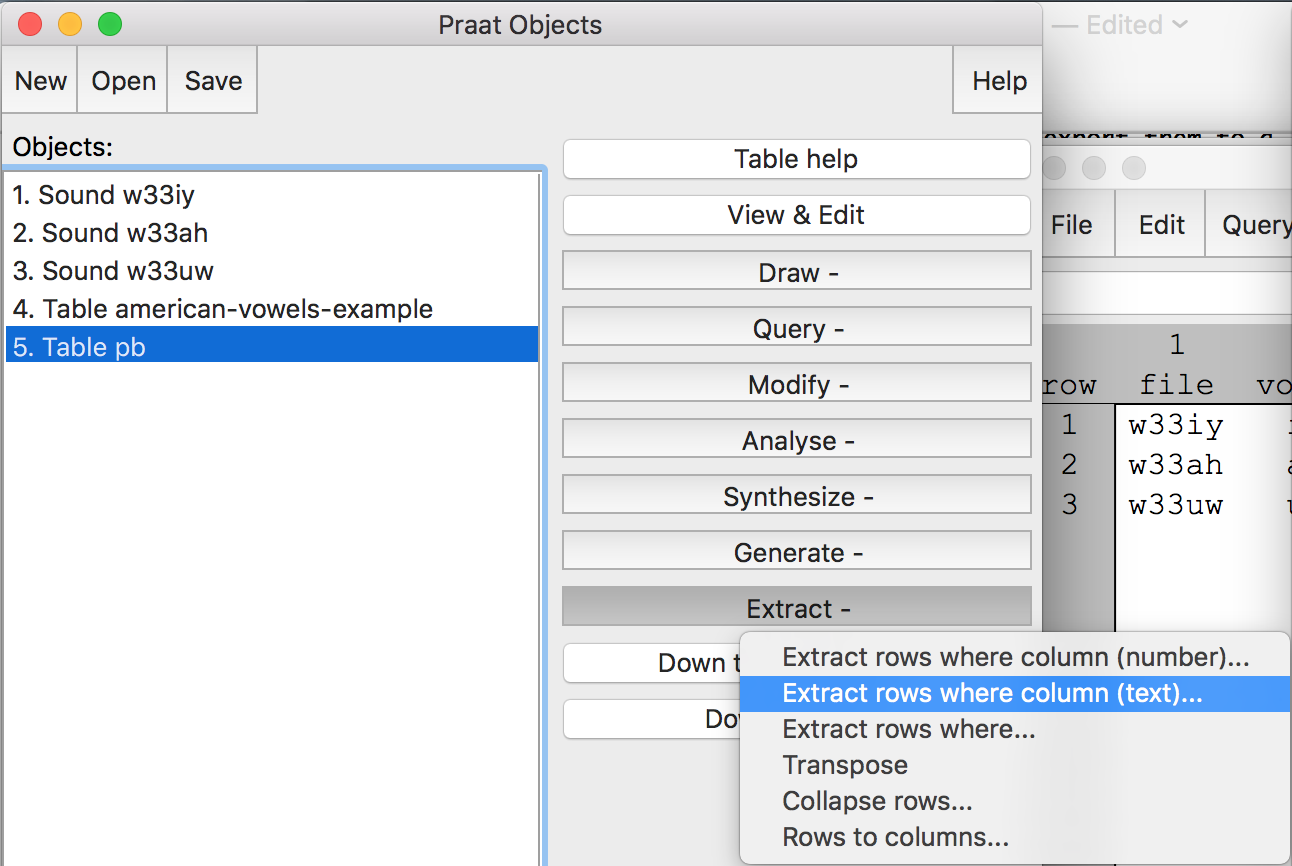
\includegraphics[width=0.8\textwidth]{./figures/Praat-20-Extract-rows-pb}
	\end{center}
\end{figure}
%
\item This should open a dialog window asking which rows to extract. The goal here is to extract the data only from the group of people you analyzed. Thus, if you analyzed the data from a male individual, you extract the data from only the male participants in the dataset. Conversely, if you analyzed the data from a female individual, you should extract only the data from the female participants in the dataset. You can extract the correct rows by setting \softmenu{Extract all rows where column is\ldots} to \emph{Type}, select \softmenu{is equal to} and set \softmenu{the text} to \emph{w} if you want to extract only the data from the females in the dataset, and to \emph{m} if you want to extract the data from the males (see figure~\ref{praat-pb-table-extract-w} for example).
%
\begin{figure}[!tbp]
\caption{\Praat{} -- Extracting the data from the females in the Peterson \& Barney 1952 data}
\label{praat-pb-table-extract-w}
	\begin{center}
		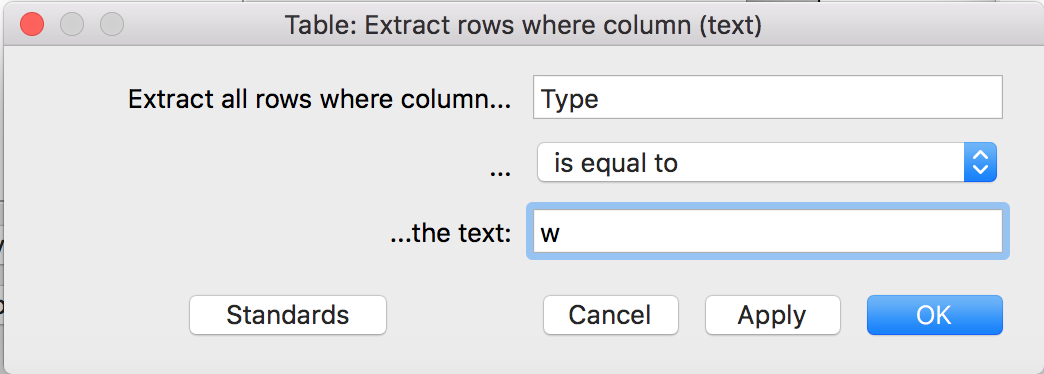
\includegraphics[width=0.8\textwidth]{./figures/Praat-21-table-extract}
	\end{center}
\end{figure}
%
\item You should now have another copy of the \emph{Table pb} with only the data you selected included.
%
\item Choose this new table and click on \softmenu{Draw} $>$ \softmenu{Draw Ellipses} (figure~\ref{praat-pb-draw-ellipses}).
%
\begin{figure}[!tbp]
\caption{\Praat{} -- Drawing ellipses in F1--F2 space for each vowel category in the Peterson \& Barney 1952 data --  data from females only}
\label{praat-pb-draw-ellipses}
	\begin{center}
		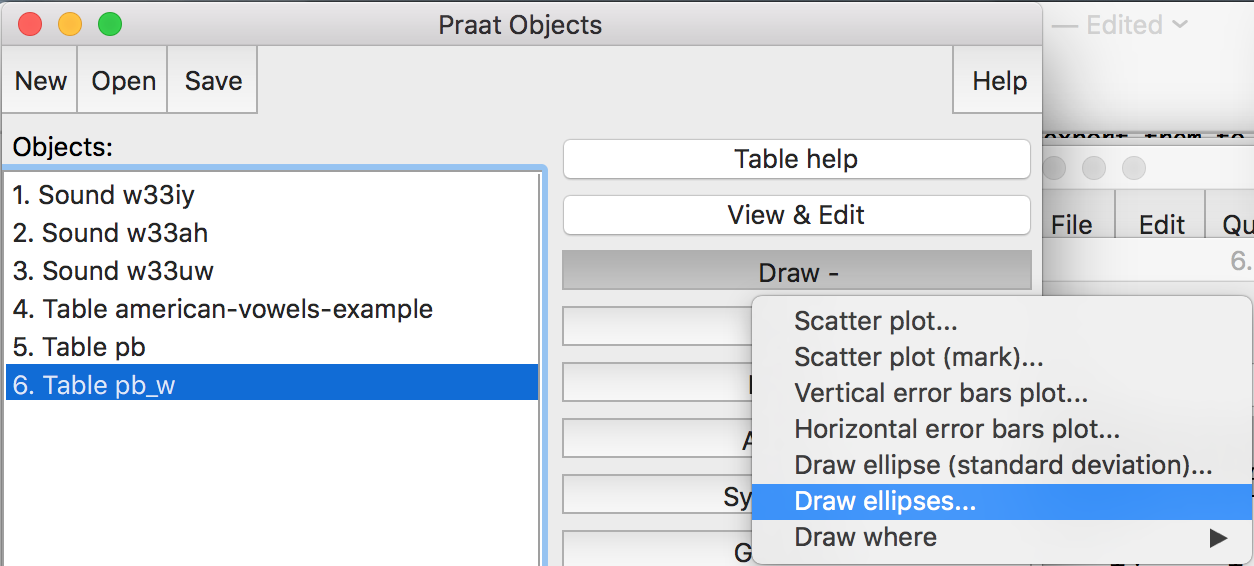
\includegraphics[width=0.8\textwidth]{./figures/Praat-22-Draw-ellipses}
	\end{center}
\end{figure}
%
\item This will open a dialog box much like the one you used to input your original plot's parameters. Use the same parameters here, but change the \softmenu{Number of sigmas} to \emph{2}. This will create ellipses capturing 2 standard deviations of F1 and F2 values in the dataset (figure~\ref{praat-pb-draw-ellipses-dialog}).
%
\begin{figure}[!tbp]
\caption{\Praat{} -- Drawing 2 Standard Deviation ellipses in F1--F2 space for each vowel category in the Peterson \& Barney 1952 data --  data from females only}
\label{praat-pb-draw-ellipses-dialog}
	\begin{center}
		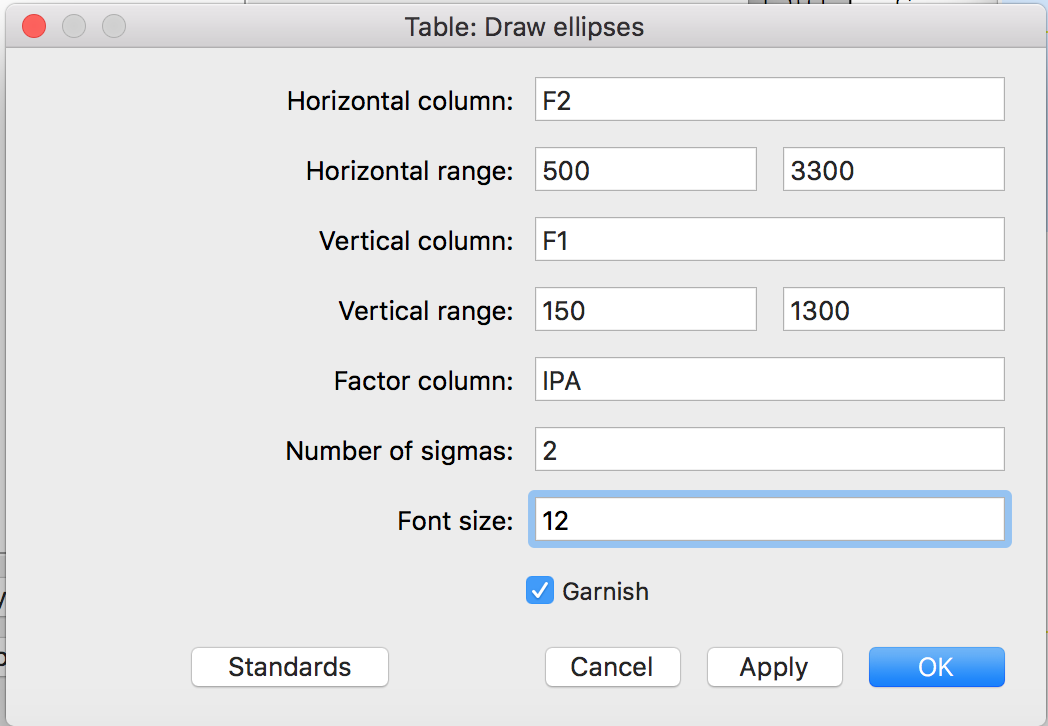
\includegraphics[width=0.8\textwidth]{./figures/Praat-23-Draw-ellipses-dialog}
	\end{center}
\end{figure}
%
\item You will produce a figure like figure~\ref{praat-pb-draw-ellipses-output}.
%
\begin{figure}[!tbp]
\caption{\Praat{} -- Ellipses capturing 2 standard deviations in the F1--F2 space for each vowel category in the Peterson \& Barney 1952 data --  data from females only}
\label{praat-pb-draw-ellipses-output}
	\begin{center}
		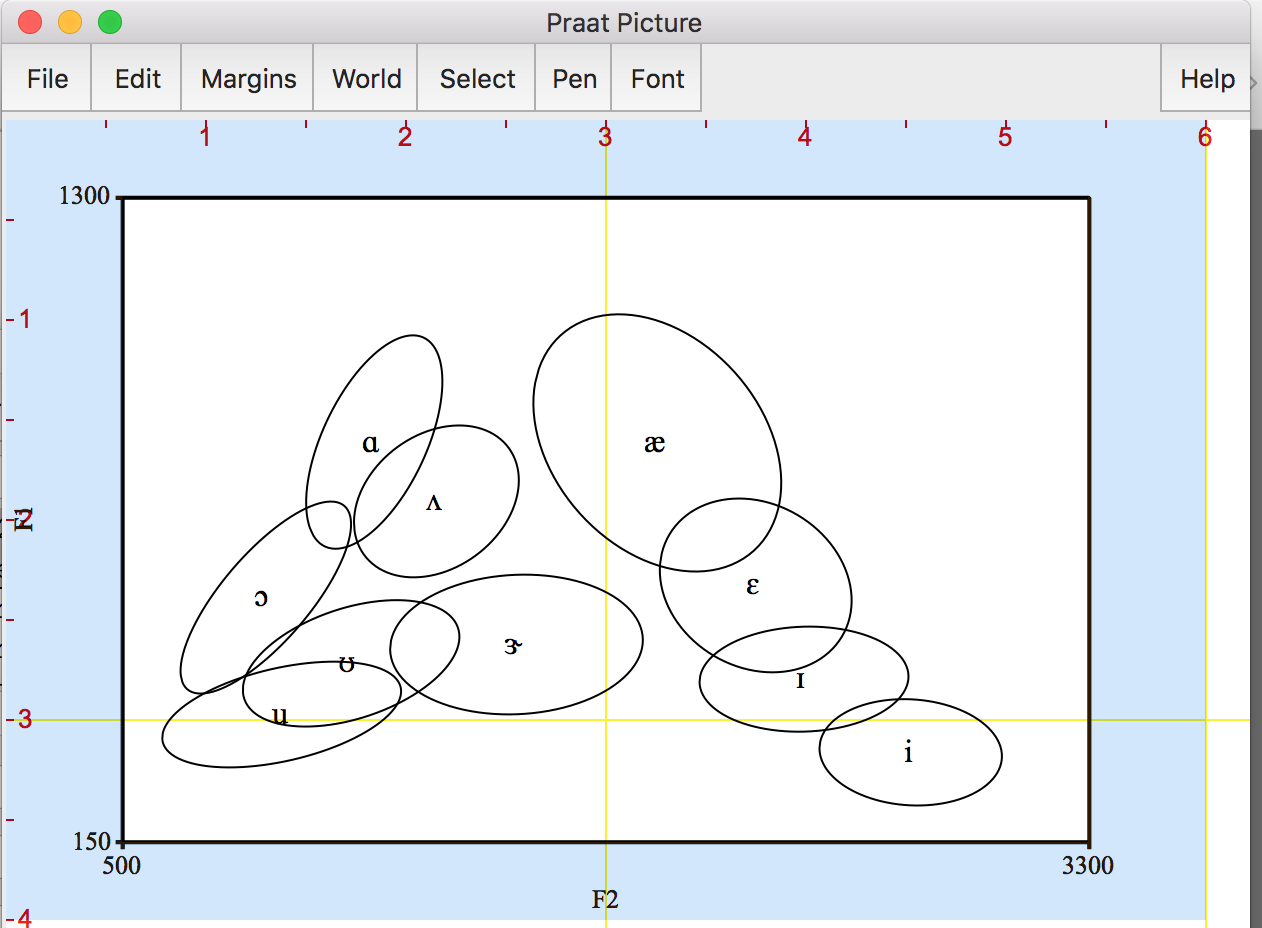
\includegraphics[width=0.8\textwidth]{./figures/Praat-24-Ellipses}
	\end{center}
\end{figure}
%
\end{enumerate}

With this figure in hand, you can start answering the question of whether the pattern you observed in the data from the single participant you analyzed holds across multiple participants. Does it? In what way? Does this new pattern present any challenges to the idea that there are one--to--one mappings between the acoustic and articulatory representations of vowels?

\paragraph{Putting the graph in context, part II.} Finally, you can try to visualize how the data you originally observed would look like when overlaid on the plot you just produced. You should first change the plot color to red (or another color of your choice) by going to the \softmenu{Pen} $>$ \softmenu{Red}, in the \softmenu{Picture} window (figure~\ref{praat-change-color}). Then, you should select the table containing your data from the \softmenu{Objects} list (if your data is not there anymore, you will need to reload it), and recreate the plot of the F1 and F2 values you measured. If you use the same ranges for both axes and uncheck the option \softmenu{Garnish}, you should just plot in red the original data you measured on top of the larger dataset of \citeA{peterson1952}. I will not show you what this figure would look like, since at this point you should be able to produce it by yourself.


\begin{figure}[!tbp]
\caption{\Praat{} -- Changing the plot color for overlaying a new plot on top of an existing one.}
\label{praat-change-color}
	\begin{center}
		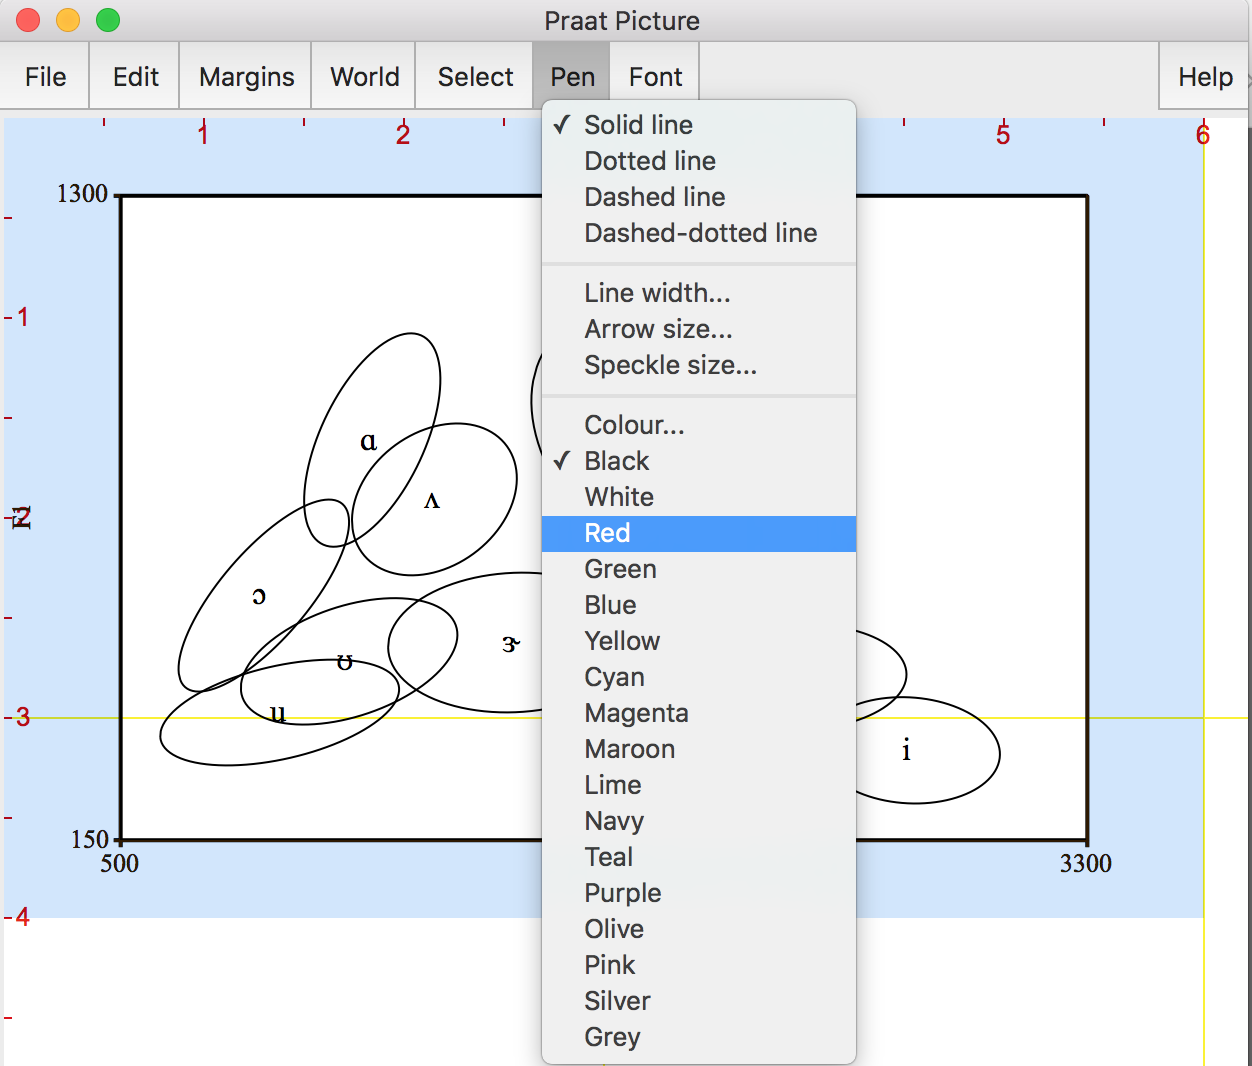
\includegraphics[width=0.8\textwidth]{./figures/Praat-25-Change-color}
	\end{center}
\end{figure}

Once you create this new figure, you are finally in a position to see how the data you analyzed fit within the larger dataset of F1--F2 values for American English vowels. Do all your observations fit within the 2 standard deviation ellipses? Do they happen to fit into another vowel category's ellipsis? Finally, what does this final plot tell you about the potential of there being a simple one--to--one mapping between simple acoustic features and articulatory representations of vowels? Can you think of any way in which this could be improved upon?

\subsection{What you should hand in.}

\begin{enumerate}
%
\item The formant values you measured. This could easily be done by including the \filefmat{csv} file you used to read your data into \Praat{} into your final submission.
%
\item A short write up of your efforts and your major conclusions based on the data you analyzed and graphed during this lab. You should use the questions I present to you in each section as a way of structuring your report. This report should also contain:
% 
   \begin{enumerate}
   %
   \item A plot of the formant values of each vowel you measured (all in one plot), a small description of how you obtained them (did you use Praat's formant track function or did you use the mouse cursor?), the problems you encountered and how you overcame them. Try to motivate your decisions during the process. It would also be best if you selected the most informative version of this plot you could make.
   %
   \item A plot of the 2 standard deviation ellipses for the relevant group of individuals in the \citeA{peterson1952}'s dataset (males, if you analyzed the data from a male, females otherwise).
   %
   \item A plot overlaying the data you originally measured on top of the plot described immediately above.
   %
   \end{enumerate}
%
\end{enumerate}

\subsection{Deadline}

This part of the lab (part A) is due by \emph{Monday, February 19th, by midnight}, via the NYUClasses web interface. You should create a zip file containing your write up and the \filefmat{csv} file you created with your F1 and F2 measurements.

There will \emph{no penalties} for handing in this part of the lab after the deadline, however, as it was \emph{my fault} that you received this assignment late. Therefore, for this part of the lab, even if you hand it in late, you will have it back as soon as possible.
